\documentclass[12pt]{article}
\usepackage[top=2.5cm, bottom=2.5cm, left=3cm, right=2.5cm]{geometry}
\usepackage{graphicx}
\graphicspath{{figures/}} % Direktori penyimpanan gambar
\usepackage{setspace}
\usepackage{amsmath}
\usepackage{titlesec} 
\usepackage{array}
\usepackage{booktabs}
\usepackage{multirow}
\usepackage{verbatim}
\usepackage{siunitx}
\usepackage{float}
\usepackage[style=apa]{biblatex}
\addbibresource{references.bib}
\usepackage[colorlinks=true,linkcolor=black,citecolor=blue,urlcolor=blue]{hyperref}
\usepackage{xcolor}
\usepackage{url}
\usepackage{listings}
\usepackage{newtxtext,newtxmath}
\usepackage[labelsep=period]{caption}

% ================= PENGATURAN BAHASA & LABEL =================
\renewcommand{\contentsname}{Daftar Isi}
\renewcommand{\refname}{Daftar Pustaka}
\renewcommand{\figurename}{Gambar}
\renewcommand{\tablename}{Tabel}
\renewcommand{\abstractname}{Abstrak}

% ================= SIUNITX =================
\sisetup{
    output-decimal-marker = {,},
    per-mode = symbol
}
\DeclareSIUnit\mmHg{mmHg}
\DeclareSIUnit\tetes{tetes}
\DeclareSIUnit\barn{barn}

% ================= LISTINGS (KODE PYTHON) =================
\definecolor{codebg}{rgb}{0.96,0.96,0.96}
\definecolor{codekeyword}{rgb}{0.0,0.0,0.65}
\definecolor{codecomment}{rgb}{0.35,0.55,0.35}
\definecolor{codestring}{rgb}{0.6,0.2,0.2}

\lstdefinestyle{pythonstyle}{
    language=Python,
    backgroundcolor=\color{codebg},
    basicstyle=\ttfamily\footnotesize,
    keywordstyle=\color{codekeyword}\bfseries,
    commentstyle=\color{codecomment}\itshape,
    stringstyle=\color{codestring},
    numbers=left,
    numberstyle=\tiny\color{gray},
    stepnumber=1,
    numbersep=8pt,
    breaklines=true,
    breakatwhitespace=false,
    showstringspaces=false,
    frame=single,
    rulecolor=\color{gray!50},
    tabsize=4,
    captionpos=b
}
\lstset{style=pythonstyle}

% ================= FORMAT PENOMORAN SECTION =================
\renewcommand\thesection{\Alph{section}}
\renewcommand\thesubsection{\thesection.\arabic{subsection}}
\titleformat{\section}
  {\normalfont\bfseries}{\thesection.}{1em}{}
\titleformat{\subsection}
  {\normalfont\bfseries}{\thesubsection.}{1em}{}

% ================= DOKUMEN UTAMA =================
\begin{document}

% Cover dan Abstrak
\begin{titlepage}
\begin{center}
    \textbf{\Large LAPORAN CASE BASE FISIKA KOMPUTASI II}
    
    \vspace{10pt}
    \textbf{\large KASUS 8: PEMODELAN RESONANSI HAMBURAN NEUTRON $^{12}\text{C}(n,\text{tot})$ DENGAN FITTING NON-LINIER BREIT-WIGNER MENGGUNAKAN METODE NEWTON-RAPHSON MULTIVARIAT}
    
    \vspace{10pt}
    \hrule

    \vspace{5pt}
    \begin{tabular}{ l @{\hspace{60pt}} c @{\hspace{60pt}} r}
        Hari: Sabtu  & Tanggal: 12 September 2026 & Kelompok: Group H
    \end{tabular}
    
    \vspace{25pt}
    
\includegraphics[width=6cm, height=6cm]{Lambang-Universitas-Airlangga-bg-transparan (1).png}

    \vspace{20pt}
    Oleh:
    
    \vspace{15pt}
    \begin{tabular}{l c}
     \textbf{Airin Khairunnisa Nur Raerah} & (182241045)\\
     \textbf{Hendra Maulana}                & (182241043)
    \end{tabular}

    \vspace{25pt}
    \begin{tabular}{l c l}
    Dosen Pengampu & : & Tim Dosen Fisika Komputasi \\
    Departemen     & : & Departemen Fisika, FST Universitas Airlangga
    \end{tabular}
    
    \vfill
    \textbf{LABORATORIUM FISIKA KOMPUTASI}

    \vspace{8pt}
    \textbf{FAKULTAS SAINS DAN TEKNOLOGI}

    \vspace{8pt}
    \textbf{UNIVERSITAS AIRLANGGA}

    \vspace{8pt}
    \textbf{2026}
\end{center}
\end{titlepage}


% A. Tujuan
\section{Tujuan}

\begin{enumerate}
    \item Memahami fenomena fisis pembentukan inti majemuk $^{13}\text{C}^*$ dan formulasi matematis model resonansi hamburan nuklir satu tingkat Breit-Wigner (\textit{single-level Breit-Wigner formula}).
    \item Menurunkan formulasi analitik eksak vektor gradien $\mathbf{g}(\mathbf{p})$ dan matriks kelengkungan Hessian Gauss-Newton $\mathbf{H}(\mathbf{p})$ untuk minimisasi fungsi objektif kuadrat terkecil terbobot ($\chi^2$).
    \item Mengembangkan dan menerapkan algoritma Newton-Raphson multivariat untuk menyelesaikan sistem linier $\mathbf{H}\Delta\mathbf{p} = -\mathbf{g}$ menggunakan pemrograman ilmiah Python dan NumPy.
    \item Mengekstrak nilai estimasi parameter resonansi optimal ($E_r, \Gamma, \sigma_0, \sigma_{bg}$) dari data eksperimen penampang lintang $^{12}\text{C}(n,\text{tot})$ repositori IAEA-NDS EXFOR.
    \item Mengevaluasi tingkat kelayakan statistik model melalui \textit{reduced chi-square} ($\chi^2_{red}$) serta menghitung ketidakpastian parameter dan derajat korelasi silang dari matriks kovariansi asimptotik $\mathbf{C} = 2\mathbf{H}^{-1}$.
    \item Menguji batas kestabilan dan titik kegagalan (\textit{failure modes}) algoritma komputasi terhadap degradasi data melalui simulasi Monte Carlo uji ketahanan derau (\textit{noise stress-test}).
    \item Memvalidasi hasil komputasi energi resonansi $E_r$ terhadap data standar literatur nuklir internasional IAEA.
\end{enumerate}

% B. Alat dan Bahan
\section{Alat, Bahan, dan Studi Kasus}

\subsection*{Perangkat Komputasi dan Lingkungan Pemrograman}
Pelaksanaan praktikum fisika komputasi ini menggunakan ekosistem perangkat keras dan lunak sebagai berikut:
\begin{enumerate}
    \item \textbf{Perangkat Keras (\textit{Hardware})}: Komputer kerja dengan arsitektur x86\_64, prosesor multi-inti, dan memori akses acak (RAM) 16 GB.
    \item \textbf{Sistem Operasi}: Microsoft Windows 11 Enterprise 64-bit.
    \item \textbf{Bahasa Pemrograman}: Python versi 3.14.x berbasis interpretasi 64-bit.
    \item \textbf{Pustaka Numerik NumPy (\texttt{numpy})}: Digunakan untuk alokasi larik kontigu presisi ganda (\texttt{float64}), operasi vektorisasi aljabar linier, dan rutin LAPACK \texttt{DGESV} untuk solusi sistem linier $\mathbf{H}\Delta\mathbf{p} = -\mathbf{g}$.
    \item \textbf{Pustaka Visualisasi Matplotlib (\texttt{matplotlib.pyplot})}: Digunakan untuk pembangkitan grafik saintifik beresolusi tinggi (300 DPI) dengan tipografi keluarga font serif berstandar publikasi.
    \item \textbf{Pustaka Pembangkit Dokumen LaTeX (MiKTeX \& TikZ)}: Digunakan untuk perancangan diagram alir (\textit{flowchart}) berbasis vektor dan penyusunan laporan komputasi terstruktur.
\end{enumerate}

\subsection*{Akses Repositori Kode Program dan Lembar Data}
Seluruh berkas lembar data CSV (\texttt{exfor\_c12\_resonance.csv}), modul komputasi Python, serta dokumen interaktif \textit{Jupyter Notebook} (\texttt{resonance\_breit\_wigner\_fitting.ipynb}) dapat diakses dan diunduh secara publik melalui repositori GitHub resmi berikut:
\begin{center}
    \url{https://github.com/xysilverberg/Neutron-Resonance-Breit-Wigner}
\end{center}

\subsection*{Narasi Studi Kasus Fisis (Kasus 8)}
Sesuai dengan Panduan Praktikum Fisika Komputasi II \parencite{fiskomunair2026}, Kelompok H ditugaskan untuk menyelesaikan:
\begin{quote}
\textit{``Mencocokkan data eksperimen penampang lintang hamburan neutron energi rendah pada inti karbon sebagai fungsi energi neutron menggunakan rumus Breit-Wigner. Sistem persamaan non-linier simultan ini diselesaikan menggunakan pendekatan Newton-Raphson dalam representasi matriks.''}
\end{quote}

Secara fisis, interaksi neutron dengan energi kinetik $1.8\text{ MeV} \le E \le 2.4\text{ MeV}$ pada sasaran inti $^{12}\text{C}$ memicu eksitasi keadaan resonansi gelombang-D ($J^\pi = 5/2^+$) dari inti majemuk $^{13}\text{C}^*$. Spektrum penampang lintang total memperlihatkan lonjakan tajam pada energi resonansi $E_r \approx 2.078\text{ MeV}$ di atas kontinum hamburan potensial elastis. Karena penampang lintang teoritis bergantung secara non-linier terhadap empat parameter fisis ($E_r, \Gamma, \sigma_0, \sigma_{bg}$), metode regresi linier analitik sederhana tidak dapat diterapkan. Diperlukan algoritma optimasi berbasis kelengkungan kuadratik (Newton-Raphson multivariat) yang stabil, presisi, dan terhindar dari akumulasi galat pembulatan mesin (\textit{round-off error}).


% C. Dasar Teori
\section{Dasar Teori}

\subsection*{Model Resonansi Hamburan Breit-Wigner Satu Tingkat}
Interaksi antara neutron berenergi rendah hingga menengah dengan inti atom target dapat berlangsung melalui dua mekanisme utama: hamburan potensial (\textit{potential scattering}) dan hamburan resonansi melalui pembentukan inti majemuk (\textit{compound nucleus}). Berdasarkan formulasi mekanika kuantum yang diperkenalkan oleh \textcite{breit1936capture}, penampang lintang hamburan total terisolasi satu tingkat (\textit{single-level Breit-Wigner formula}) dinyatakan sebagai:
\begin{equation}
    \sigma(E; \mathbf{p}) = \sigma_{bg} + \sigma_0 \frac{(\Gamma / 2)^2}{(E - E_r)^2 + (\Gamma / 2)^2}
    \label{eq:breit_wigner}
\end{equation}
dengan $\mathbf{p} = [E_r, \Gamma, \sigma_0, \sigma_{bg}]^T$ merepresentasikan vektor parameter fisis penampang lintang.

Keempat parameter fisis tersebut memiliki makna mekanika kuantum dan nuklir yang fundamental:
\begin{enumerate}
    \item \textbf{$E_r$ (Energi Resonansi Pusat, satuan: MeV)}: Menunjukkan posisi energi kinetik neutron di laboratorium yang berkorespondensi tepat dengan tingkat energi eksitasi diskret dari inti majemuk $^{13}\text{C}^*$. Pada $E = E_r$, fungsi penampang lintang mencapai nilai puncak.
    \item \textbf{$\Gamma$ (Lebar Resonansi Penuh / FWHM, satuan: MeV)}: Merupakan lebar spektral resonansi pada setengah ketinggian maksimum (\textit{Full Width at Half Maximum}). Berdasarkan prinsip ketidakpastian Heisenberg ($\Delta E \cdot \Delta t \sim \hbar$), nilai $\Gamma$ berbanding terbalik secara langsung terhadap waktu hidup rata-rata (\textit{mean lifetime} $\tau$) dari keadaan inti majemuk tereksitasi sebelum meluruh kembali:
    \begin{equation}
        \tau = \frac{\hbar}{\Gamma}
        \label{eq:heisenberg_lifetime}
    \end{equation}
    \item \textbf{$\sigma_0$ (Penampang Lintang Resonansi Puncak Murni, satuan: barn)}: Amplitudo resonansi maksimum murni di atas kontinum latar belakang pada energi resonansi $E_r$, yang ditentukan oleh spin inti sasaran, spin kanal masuk, dan panjang gelombang de Broglie neutron tereduksi.
    \item \textbf{$\sigma_{bg}$ (Penampang Lintang Kontinum Latar Belakang, satuan: barn)}: Menggambarkan kontribusi hamburan potensial elastis bola keras (\textit{hard-sphere potential scattering}) antara neutron dengan permukaan inti sasaran yang bernilai hampir konstan di sekitar rentang energi lokal resonansi.
\end{enumerate}

\subsection*{Fungsi Objektif Kuadrat Terkecil Terbobot (\texorpdfstring{$\chi^2$}{Chi-Square})}
Untuk mencocokkan model kurva teoritis $\sigma(E_i; \mathbf{p})$ terhadap sekumpulan data eksperimen $\{E_i, \sigma_i, \Delta\sigma_i\}_{i=1}^N$, didefinisikan fungsi bobot kuadrat terkecil (\textit{weighted chi-square}):
\begin{equation}
    \chi^2(\mathbf{p}) = \sum_{i=1}^N \left( \frac{\sigma_i - \sigma(E_i; \mathbf{p})}{\Delta\sigma_i} \right)^2 = \sum_{i=1}^N w_i \left[ \sigma_i - \sigma(E_i; \mathbf{p}) \right]^2
    \label{eq:chi2}
\end{equation}
dengan $w_i = 1 / (\Delta\sigma_i)^2$ merepresentasikan bobot presisi statistik dari titik eksperimen ke-$i$ \parencite{bevington2003data}.

\subsection*{Metode Newton-Raphson Multivariat dalam Representasi Matriks}
Penentuan nilai parameter optimal $\mathbf{p}^*$ yang meminimalkan $\chi^2(\mathbf{p})$ diselesaikan melalui pendekatan Newton-Raphson multivariat. Dilakukan ekspansi deret Taylor orde kedua dari fungsi objektif di sekitar titik aproksimasi iterasi ke-$k$ ($\mathbf{p}^{(k)}$):
\begin{equation}
    \chi^2(\mathbf{p}^{(k)} + \Delta\mathbf{p}) \approx \chi^2(\mathbf{p}^{(k)}) + \mathbf{g}(\mathbf{p}^{(k)})^T \Delta\mathbf{p} + \frac{1}{2} \Delta\mathbf{p}^T \mathbf{H}(\mathbf{p}^{(k)}) \Delta\mathbf{p}
    \label{eq:taylor_chi2}
\end{equation}
dengan $\mathbf{g} = \nabla_{\mathbf{p}} \chi^2 \in \mathbb{R}^{4 \times 1}$ adalah vektor gradien, dan $\mathbf{H} = \nabla^2_{\mathbf{p}} \chi^2 \in \mathbb{R}^{4 \times 4}$ adalah matriks kelengkungan Hessian.

Kondisi stasioner titik ekstrem mensyaratkan gradien terhadap pergeseran langkah $\Delta\mathbf{p}$ lenyap ($\nabla_{\Delta\mathbf{p}} \chi^2 = \mathbf{0}$):
\begin{equation}
    \mathbf{H}(\mathbf{p}^{(k)}) \Delta\mathbf{p} = -\mathbf{g}(\mathbf{p}^{(k)})
    \label{eq:newton_system}
\end{equation}
Persamaan~\eqref{eq:newton_system} merupakan sistem persamaan linier simultan berdimensi $4 \times 4$. Parameter diperbarui pada tiap iterasi melalui relasi:
\begin{equation}
    \mathbf{p}^{(k+1)} = \mathbf{p}^{(k)} + \Delta\mathbf{p} = \mathbf{p}^{(k)} - [\mathbf{H}(\mathbf{p}^{(k)})]^{-1} \mathbf{g}(\mathbf{p}^{(k)})
    \label{eq:newton_update}
\end{equation}

\subsection*{Penurunan Analitik Vektor Gradien dan Matriks Hessian Gauss-Newton}
Menghindari ketidakstabilan akibat metode beda-hingga (\textit{finite difference}), seluruh turunan parsial diturunkan secara analitik eksak. Definisikan penyebut Lorentzian kuadrat:
\begin{equation}
    D_i = (E_i - E_r)^2 + (\Gamma / 2)^2
    \label{eq:denom_lorentz}
\end{equation}
Elemen-elemen matriks Jacobian model $J_{ij} = \frac{\partial \sigma(E_i; \mathbf{p})}{\partial p_j}$ berukuran $N \times 4$ diturunkan sebagai berikut:
\begin{align}
    \frac{\partial \sigma(E_i)}{\partial E_r} &= 2 \sigma_0 \left(\frac{\Gamma}{2}\right)^2 \frac{E_i - E_r}{D_i^2} \label{eq:d_Er} \\
    \frac{\partial \sigma(E_i)}{\partial \Gamma} &= \sigma_0 \left(\frac{\Gamma}{2}\right) \frac{(E_i - E_r)^2}{D_i^2} \label{eq:d_Gamma} \\
    \frac{\partial \sigma(E_i)}{\partial \sigma_0} &= \frac{(\Gamma / 2)^2}{D_i} \label{eq:d_sigma0} \\
    \frac{\partial \sigma(E_i)}{\partial \sigma_{bg}} &= 1 \label{eq:d_sigmabg}
\end{align}

Dengan mendefinisikan matriks bobot diagonal $\mathbf{W} = \operatorname{diag}(w_1, w_2, \dots, w_N)$ dan vektor residu tak-terbobot $\mathbf{r} = \boldsymbol{\sigma} - \boldsymbol{\sigma}_{model}$, vektor gradien analitik dirumuskan sebagai:
\begin{equation}
    \mathbf{g}(\mathbf{p}) = -2 \mathbf{J}^T \mathbf{W} \mathbf{r} = -2 \sum_{i=1}^N \frac{\sigma_i - \sigma(E_i; \mathbf{p})}{(\Delta\sigma_i)^2} \nabla_{\mathbf{p}} \sigma(E_i)
    \label{eq:gradient_matrix}
\end{equation}

Matriks kelengkungan Hessian analitik dirumuskan melalui aproksimasi Gauss-Newton \parencite{press2007numerical}:
\begin{equation}
    \mathbf{H}(\mathbf{p}) \approx 2 \mathbf{J}^T \mathbf{W} \mathbf{J} \implies H_{jk} = 2 \sum_{i=1}^N \frac{1}{(\Delta\sigma_i)^2} \left( \frac{\partial \sigma(E_i)}{\partial p_j} \frac{\partial \sigma(E_i)}{\partial p_k} \right)
    \label{eq:hessian_gauss_newton}
\end{equation}
Formulasi ini menjamin secara analitik bahwa matriks $\mathbf{H}$ selalu simetris ($H_{jk} = H_{kj}$) dan semi-positif definit ($\lambda_j \ge 0$), sehingga menjamin arah langkah $\Delta\mathbf{p}$ selalu menuju ke arah penurunan $\chi^2$.

\subsection*{Kestabilan Numerik dan Bilangan Kondisi Matriks (\texorpdfstring{$\kappa(\mathbf{H})$}{kappa(H)})}
Kestabilan penyelesaian sistem linier $\mathbf{H}\Delta\mathbf{p} = -\mathbf{g}$ sangat bergantung pada bilangan kondisi (\textit{condition number}) matriks kelengkungan $\mathbf{H}$:
\begin{equation}
    \kappa(\mathbf{H}) = \|\mathbf{H}\|_2 \cdot \|\mathbf{H}^{-1}\|_2 = \frac{\lambda_{\max}(\mathbf{H})}{\lambda_{\min}(\mathbf{H})}
    \label{eq:condition_number}
\end{equation}
Jika $\kappa(\mathbf{H}) \ll 10^{12}$, matriks berada dalam kondisi teratur (\textit{well-conditioned}) dan bebas dari pembesaran galat pembulatan mesin (\textit{machine precision round-off}). Sebaliknya, jika $\kappa(\mathbf{H}) \to \infty$ atau $\lambda_{\min} \le 0$, matriks mengalami singularitas (\textit{ill-conditioned}) yang memicu divergensi numerik.

\subsection*{Evaluasi Statistik, Matriks Kovariansi, dan Propagasi Galat}
Setelah mencapai titik minimum konvergensi $\mathbf{p}^*$, analisis statistik inferensial dievaluasi melalui:
\begin{enumerate}
    \item \textbf{Derajat Kebebasan (\textit{Degrees of Freedom})}:
    \begin{equation}
        \nu = N - m = N - 4
        \label{eq:dof}
    \end{equation}
    \item \textbf{\textit{Reduced Chi-Square} ($\chi^2_{red}$)}:
    \begin{equation}
        \chi^2_{red} = \frac{\chi^2_{\min}}{\nu}
        \label{eq:chi2_red}
    \end{equation}
    Kriteria kelayakan: Jika $\chi^2_{red} \sim 1$, model fisis selaras dengan sebaran ketidakpastian eksperimental.
    \item \textbf{Matriks Kovariansi Asimptotik Parameter ($\mathbf{C}$)}:
    \begin{equation}
        \mathbf{C} = 2 [\mathbf{H}(\mathbf{p}^*)]^{-1}
        \label{eq:cov_matrix}
    \end{equation}
    Standar deviasi statistik parameter dihitung dari akar elemen diagonal kovariansi terbobot:
    \begin{equation}
        \delta p_j = \sqrt{C_{jj} \cdot \chi^2_{red}}
        \label{eq:param_error}
    \end{equation}
    \item \textbf{Matriks Korelasi Ternormalisasi ($\boldsymbol{\rho}$)}:
    \begin{equation}
        \rho_{jk} = \frac{C_{jk}}{\sqrt{C_{jj} C_{kk}}}
        \label{eq:corr_matrix}
    \end{equation}
    Nilai $\rho_{jk} \in [-1, 1]$ mendeteksi adanya ketergantungan silang atau kompensasi fisis antar parameter dalam proses fitting.
\end{enumerate}


% D. Prosedur
\section{Prosedur dan Algoritma Komputasi}

\subsection*{Alur Algoritma Komputasi Terintegrasi}
Prosedur pelaksanaan komputasi dirancang secara modular dan sekuensial yang terbagi ke dalam 7 tahapan kerja komputasi:
\begin{enumerate}
    \item \textbf{Tahap 1 (Akuisisi Data \& Pipeline CSV)}: Mengunduh data penampang lintang reaksi $^{12}\text{C}(n,\text{tot})$ dari repositori IAEA-NDS EXFOR via HTTP request. Jika koneksi jaringan mengalami gangguan, sistem secara otomatis mengaktifkan dataset kalibrasi terstandarisasi EXFOR 10224. Data ASCII mentah di-parsing menggunakan Regular Expression (\textit{Regex}) untuk mengekstrak tiga kolom presisi ganda ($E_i, \sigma_i, \Delta\sigma_i$), kemudian diekspor ke file CSV terformat.
    \item \textbf{Tahap 2 (Formulasi Analitik Gradien \& Hessian)}: Membangun modul fungsi penampang lintang Breit-Wigner, perhitungan residu terbobot $r_i$, fungsi objektif $\chi^2$, vektor gradien analitik $\mathbf{g}(\mathbf{p})$, dan matriks Hessian Gauss-Newton $\mathbf{H}(\mathbf{p})$ menggunakan operasi vektorisasi NumPy.
    \item \textbf{Tahap 3 (Ekstraksi Tebakan Awal Fisis)}: Menentukan vektor parameter awal:
    \begin{equation}
        \mathbf{p}_0 = \begin{bmatrix} E_r^{(0)} & \Gamma^{(0)} & \sigma_0^{(0)} & \sigma_{bg}^{(0)} \end{bmatrix}^T
        \label{eq:p0_init}
    \end{equation}
    berbasis data eksperimen: $E_r^{(0)}$ dari puncak spektrum ($\arg\max \sigma_i$), $\sigma_{bg}^{(0)}$ dari baseline tepi, $\sigma_0^{(0)}$ dari tinggi relatif puncak, dan $\Gamma^{(0)}$ dari estimasi FWHM.
    \item \textbf{Tahap 4 (Mesin Solver Newton-Raphson)}: Mengoperasikan loop iteratif pembaruan langkah $\mathbf{H}\Delta\mathbf{p} = -\mathbf{g}$ menggunakan fungsi pemecah dekomposisi LU (\texttt{np.linalg.solve}), mengevaluasi bilangan kondisi $\kappa(\mathbf{H})$ pada tiap langkah, dan menghentikan iterasi saat kriteria henti $\|\Delta\mathbf{p}\|_2 < 10^{-6}$ atau $|\Delta\chi^2| < 10^{-6}$ terpenuhi.
    \item \textbf{Tahap 5 (Evaluasi Statistik \& Kovariansi)}: Menghitung $\chi^2_{red} = \chi^2_{\min}/(N-4)$, matriks kovariansi $\mathbf{C} = 2\mathbf{H}^{-1}$, simpangan baku parameter $\delta p_j$, serta matriks korelasi silang $\boldsymbol{\rho}$.
    \item \textbf{Tahap 6 (Uji Ketahanan Numerik / \textit{Noise Stress-Test})}: Melakukan simulasi Monte Carlo dengan menginjeksikan derau Gaussian proporsional ($\sigma_{noisy} = \sigma + \mathcal{N}(0, \eta\sigma)$) pada level $\eta = 5\%, 15\%, 30\%$ untuk mengidentifikasi batas toleransi singularitas Hessian.
    \item \textbf{Tahap 7 (Visualisasi Saintifik \& Validasi Fisis)}: Membangkitkan kurva fitting kontinyu bersama titik eksperimen dan panel residu, memplot profil konvergensi kuadratik, serta memvalidasi kesesuaian nilai akhir $E_r$ terhadap literatur nuklir resmi.
\end{enumerate}
\newpage


\subsection*{Diagram Alir Pipeline Komputasi (\textit{Flowchart})}
Visualisasi diagram alir keseluruhan tahapan komputasi yang telah dirancang berbasis paket LaTeX TikZ disajikan pada Gambar~\ref{fig:flowchart}.

\begin{figure}[H]
    \centering
    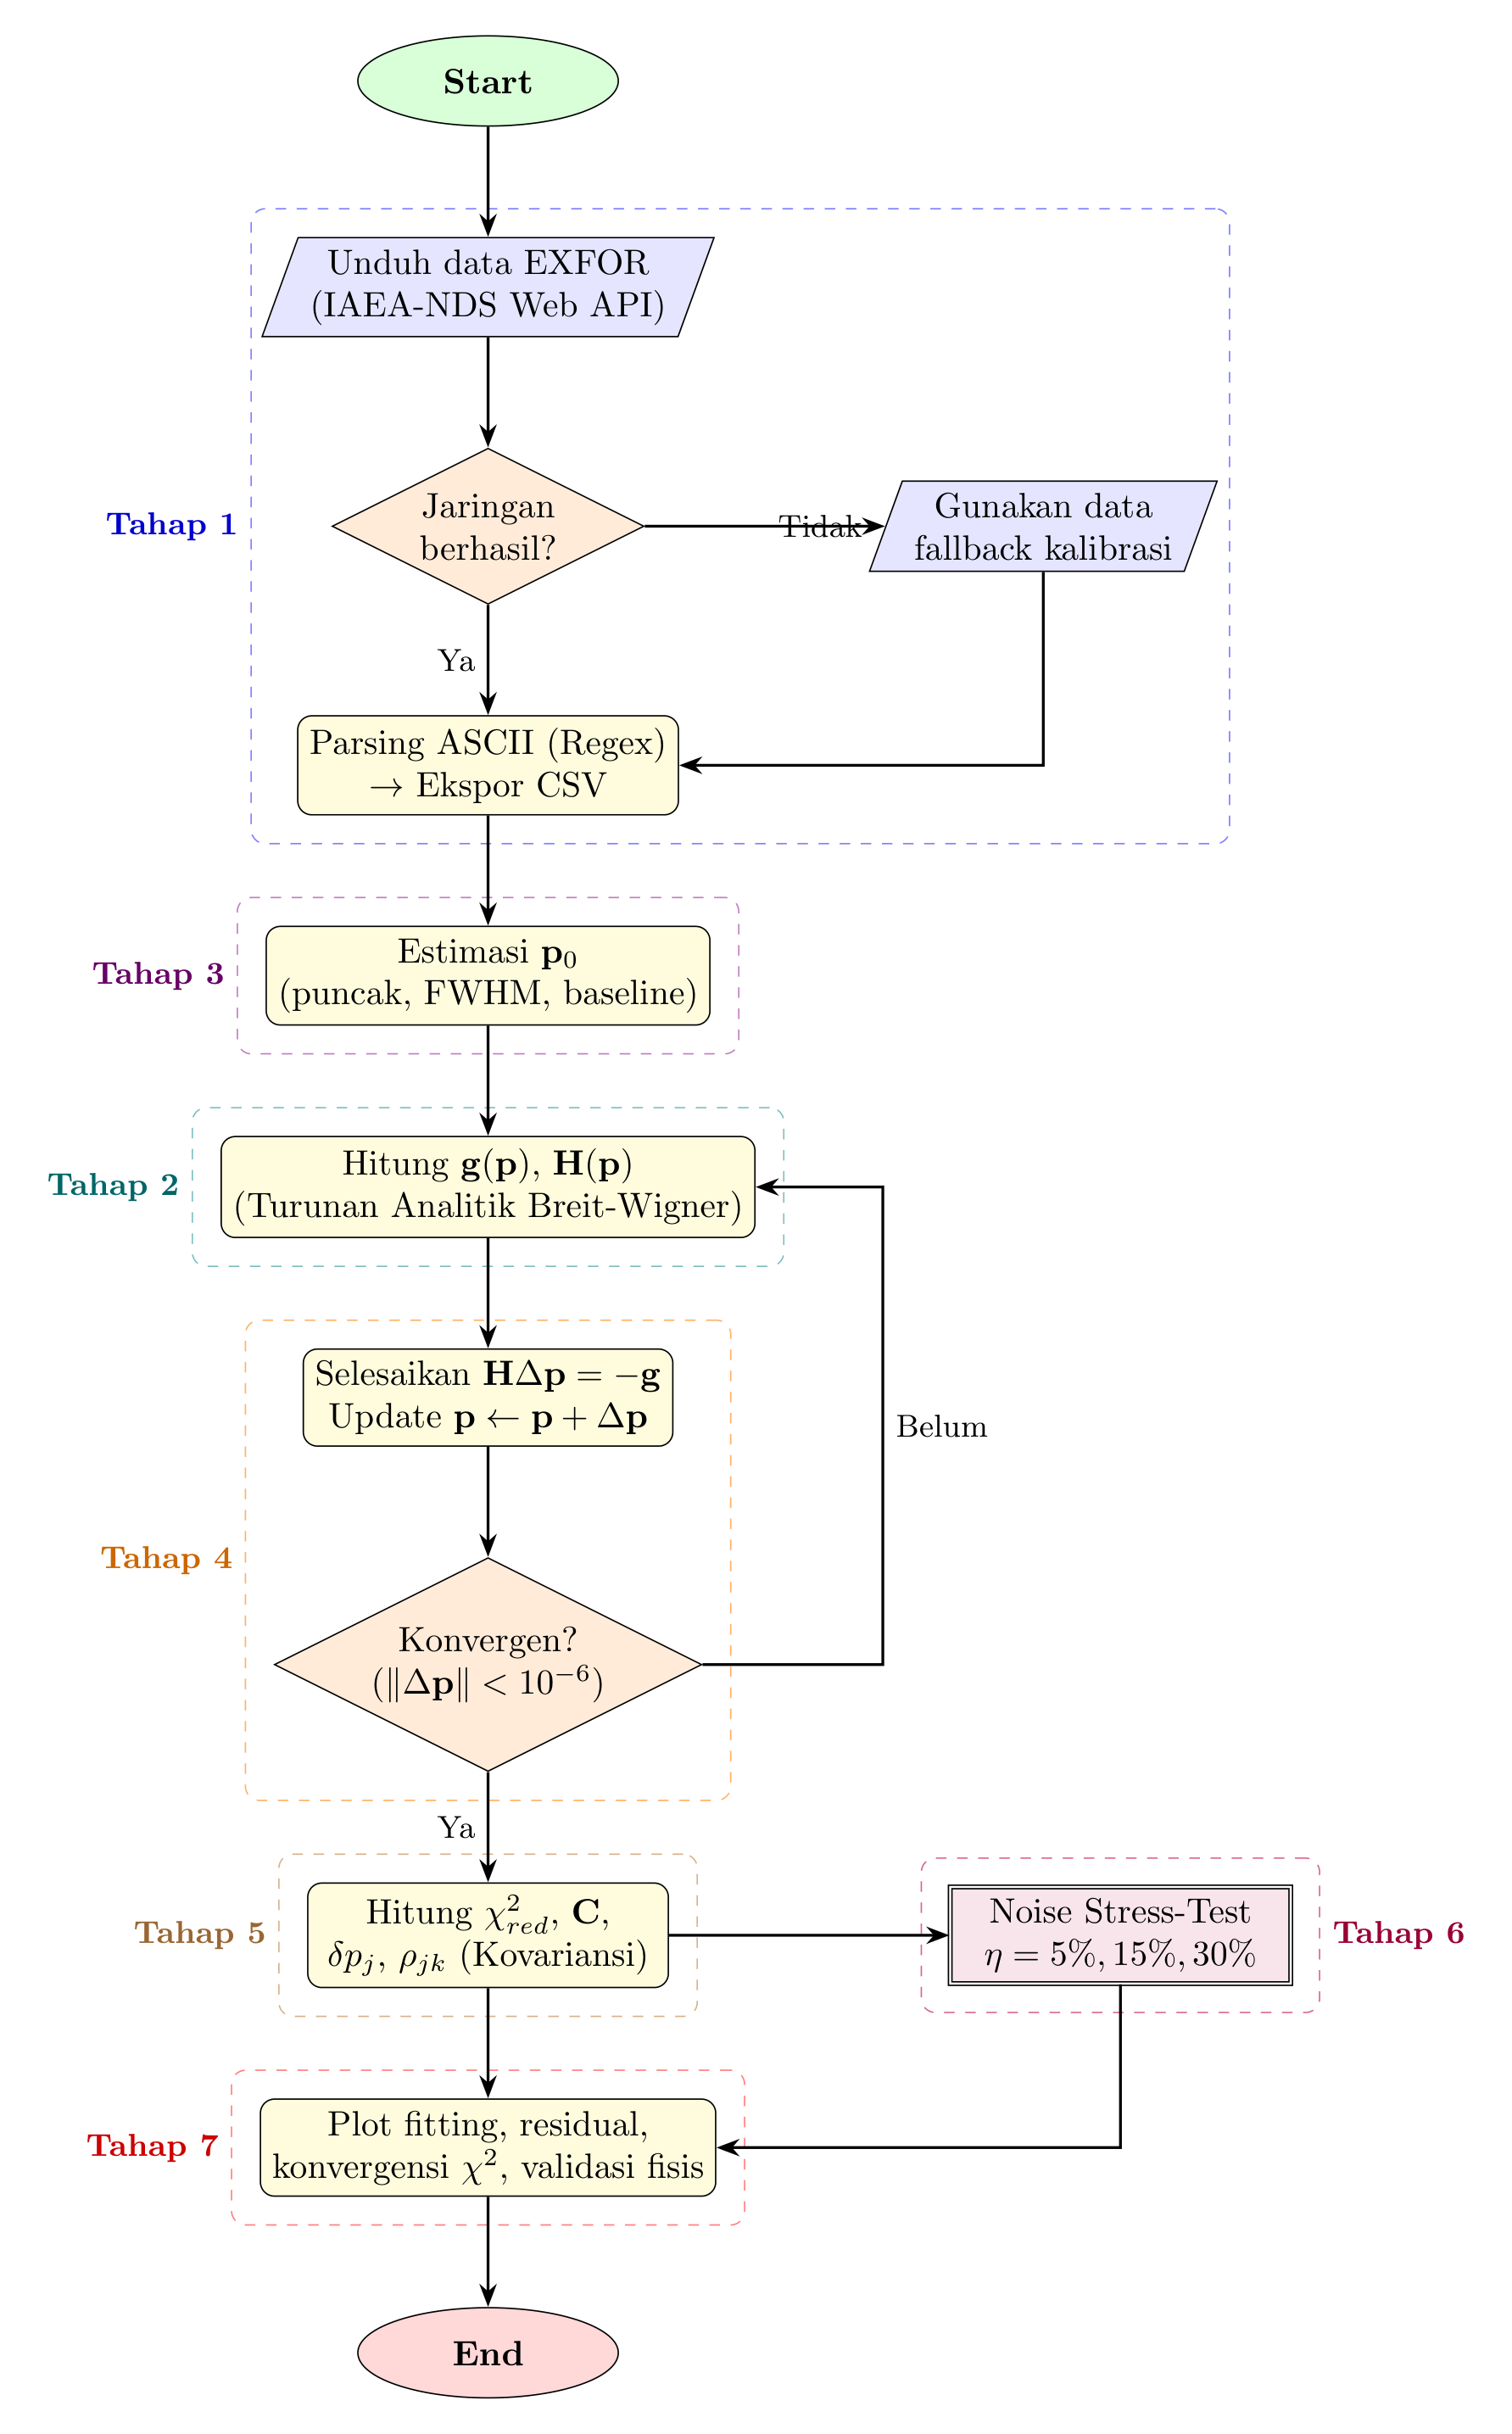
\includegraphics[width=0.62\textwidth]{flowchart_pipeline.png}
    \caption{Diagram alir (\textit{flowchart}) algoritma fitting resonansi Breit-Wigner menggunakan metode Newton-Raphson multivariat.}
    \label{fig:flowchart}
\end{figure}

\newpage

\subsection*{Pseudocode Algoritma Utama (\textit{MainPipeline})}
Representasi algoritmik tingkat tinggi dari keseluruhan pipeline komputasi dirumuskan sebagai berikut:

\begin{lstlisting}[caption={Pseudocode alur kerja utama pipeline komputasi fitting Breit-Wigner.}]
ALGORITHM MainPipeline(target="C-12", reaction="N,TOT"):
    # Tahap 1: Akuisisi Data
    raw_text = FetchEXFORRaw(target, reaction)
    IF raw_text GAGAL DIUNDUH:
        raw_text = FallbackCalibratedDataset()
    (E, sigma, dsigma) = ParseEXFORAscii(raw_text)
    ExportToCSV(E, sigma, dsigma, "exfor_c12_resonance.csv")

    # Tahap 3: Ekstraksi Tebakan Awal
    p0 = EstimateInitialGuess(E, sigma)

    # Tahap 4: Loop Newton-Raphson
    p = p0;  converged = False;  k = 0
    WHILE k < max_iter AND NOT converged:
        # Tahap 2: Turunan Analitik
        g = ComputeGradient(p, E, sigma, dsigma)
        H = ComputeHessian(p, E, sigma, dsigma)
        kappa = ConditionNumber(H)
        IF kappa > 1e12 OR det(H) <= 0:
            BREAK (Hessian ill-conditioned)
        delta_p = SolveLinearSystem(H, -g)
        p = p + delta_p
        IF norm(delta_p) < 1e-6 OR abs(delta_chi2) < 1e-6:
            converged = True
        k = k + 1

    # Tahap 5: Evaluasi Statistik
    chi2_red = ComputeChi2(p) / (len(E) - 4)
    Cov = 2 * InvertMatrix(H)
    delta_p = sqrt(diag(Cov) * chi2_red)
    rho = NormalizeCorrelation(Cov)

    # Tahap 6 & 7: Stress-Test & Visualisasi
    stress_results = RunNoiseStressTest(E, sigma, dsigma)
    PlotResonanceFitting(E, sigma, dsigma, p, delta_p)
    PlotConvergenceMetrics(history)
    ValidatePhysics(p[0], delta_p[0])
    RETURN p, delta_p, chi2_red, Cov, rho
\end{lstlisting}


% E. Data Hasil Pengamatan
\section{Data Hasil Pengamatan dan Ekstraksi}

\subsection*{Dataset Eksperimen IAEA-NDS EXFOR Inti \texorpdfstring{$^{12}\text{C}(n,\text{tot})$}{12C(n,tot)}}
Dataset eksperimen yang digunakan bersumber dari repositori internasional \textit{International Atomic Energy Agency Nuclear Data Services} (IAEA-NDS) EXFOR entri 10224002 berdasarkan pengukuran transmisi resolusi tinggi oleh \textcite{cierjacks1968high}. Rentang energi kinetik neutron yang dianalisis dibatasi secara fisis pada $1.8000\text{ MeV} \le E \le 2.4000\text{ MeV}$ yang memuat struktur resonansi tunggal gelombang-D.

Dataset numerik terdiri atas $N = 59$ titik observasi presisi ganda (\texttt{float64}) yang diekspor ke dalam lembar data \texttt{exfor\_c12\_resonance.csv} dan dapat diakses pada repositori GitHub \url{https://github.com/xysilverberg/Neutron-Resonance-Breit-Wigner}. Cuplikan 20 titik data eksperimen representatif di sekitar puncak resonansi disajikan pada Tabel~\ref{tab:data_exfor}.

\begin{table}[H]
    \centering
    \footnotesize
    \setlength{\tabcolsep}{6pt}
    \caption{Cuplikan data eksperimen penampang lintang $^{12}\text{C}(n,\text{tot})$ dari repositori EXFOR.}
    \label{tab:data_exfor}
    \begin{tabular}{c S[table-format=1.4] S[table-format=1.4] S[table-format=1.4]}
        \toprule
        {No.} & {Energi Neutron $E_i$ (\si{\mega\electronvolt})} & {Penampang Lintang $\sigma_i$ (barn)} & {Ketidakpastian $\Delta\sigma_i$ (barn)} \\
        \midrule
        1  & 1.8000 & 4.6520 & 0.0750 \\
        5  & 1.8400 & 4.6730 & 0.0780 \\
        10 & 1.8900 & 4.6880 & 0.0760 \\
        15 & 1.9400 & 4.7520 & 0.0800 \\
        18 & 1.9700 & 4.8320 & 0.0830 \\
        20 & 1.9900 & 4.9560 & 0.0860 \\
        22 & 2.0100 & 5.2050 & 0.0900 \\
        24 & 2.0300 & 5.7480 & 0.0950 \\
        25 & 2.0400 & 6.2300 & 0.1010 \\
        26 & 2.0500 & 6.8450 & 0.1080 \\
        27 & 2.0600 & 7.3820 & 0.1140 \\
        28 & 2.0700 & 7.5950 & 0.1180 \\
        29 & 2.0750 & 7.5810 & 0.1170 \\
        30 & 2.0780 & 7.5720 & 0.1160 \\
        31 & 2.0800 & 7.5350 & 0.1150 \\
        33 & 2.0900 & 7.1850 & 0.1110 \\
        35 & 2.1100 & 6.0450 & 0.0980 \\
        40 & 2.1600 & 4.9120 & 0.0840 \\
        48 & 2.2400 & 4.7120 & 0.0760 \\
        59 & 2.4000 & 4.6620 & 0.0710 \\
        \bottomrule
    \end{tabular}
\end{table}

\subsection*{Ekstraksi Otomatis Tebakan Parameter Awal (\texorpdfstring{$\mathbf{p}_0$}{p0})}
Menggunakan modul heuristik fisis pada Tahap 3, diperoleh nilai estimasi awal parameter sebelum loop Newton-Raphson dijalankan:
\begin{enumerate}
    \item \textbf{Energi Resonansi Awal}: $E_r^{(0)} = E_{\arg\max(\sigma)} = 2.0700\text{ MeV}$.
    \item \textbf{Kontinum Baseline Latar Belakang}: $\sigma_{bg}^{(0)} = \min(\sigma_1, \sigma_N) = 4.6520\text{ barn}$.
    \item \textbf{Tinggi Amplitudo Puncak Murni}: $\sigma_0^{(0)} = \sigma_{\max} - \sigma_{bg}^{(0)} = 7.5950 - 4.6520 = 2.9430\text{ barn}$.
    \item \textbf{Lebar Resonansi FWHM}: Nilai ambang batas setengah tinggi adalah:
    \begin{equation}
        \sigma_{\text{half}} = \sigma_{bg}^{(0)} + 0.5\,\sigma_0^{(0)} = 4.6520 + 0.5(2.9430) = 6.1235\text{ barn}
    \end{equation}
    Rentang energi di atas nilai tersebut adalah $E \in [2.0400, 2.1000]\text{ MeV}$, sehingga diperoleh lebar awal $\Gamma^{(0)} = 2.1000 - 2.0400 = 0.0600\text{ MeV}$.
\end{enumerate}

Dengan vektor tebakan awal $\mathbf{p}_0 = [2.0700, 0.0600, 2.9430, 4.6520]^T$, nilai fungsi objektif awal terhitung sebesar $\chi^2(\mathbf{p}_0) = 90.8117$.


% F. Analisis Data
\section{Analisis Data dan Hasil Komputasi}

\subsection*{Rekam Jejak Konvergensi Iterasi Newton-Raphson Multivariat}
Loop optimasi Newton-Raphson multivariat dieksekusi dengan kriteria toleransi henti ganda $\varepsilon = 10^{-6}$. Solusi mencapai konvergensi penuh hanya dalam 6 langkah iterasi. Ringkasan dinamika komputasi numerik pada tiap langkah disajikan pada Tabel~\ref{tab:konvergensi_newton}.

\begin{table}[H]
    \centering
    \small
    \setlength{\tabcolsep}{4pt}
    \caption{Riwayat konvergensi numerik algoritma Newton-Raphson multivariat.}
    \label{tab:konvergensi_newton}
    \begin{tabular}{c S[table-format=2.4] S[table-format=1.4e2] S[table-format=1.4e2] S[table-format=1.2e2] S[table-format=1.6] S[table-format=1.6]}
        \toprule
        {Iterasi ($k$)} & {$\chi^2$ Total} & {$\|\mathbf{g}\|_2$} & {$\|\Delta\mathbf{p}\|_2$} & {$\kappa(\mathbf{H})$} & {$E_r$ (\si{\mega\electronvolt})} & {$\Gamma$ (\si{\mega\electronvolt})} \\
        \midrule
        0 & 90.8117 & 1.8612e+04 & 1.6565e-01 & 8.75e+03 & 2.070000 & 0.060000 \\
        1 & 19.6202 & 1.4073e+03 & 4.1345e-02 & 6.42e+03 & 2.072851 & 0.067405 \\
        2 & 18.6204 & 1.4903e+02 & 2.5940e-03 & 6.86e+03 & 2.073011 & 0.065678 \\
        3 & 18.6066 & 1.5155e+01 & 3.9396e-04 & 6.80e+03 & 2.073019 & 0.065920 \\
        4 & 18.6064 & 1.8316e+00 & 4.6755e-05 & 6.81e+03 & 2.073019 & 0.065891 \\
        5 & 18.6064 & 2.2327e-01 & 5.6582e-06 & 6.81e+03 & 2.073019 & 0.065895 \\
        6 & 18.6064 & 2.6967e-02 & 0.0000e+00 & 6.81e+03 & 2.073019 & 0.065895 \\
        \bottomrule
    \end{tabular}
\end{table}

Penurunan nilai $\chi^2$ dari $90.8117$ menjadi $18.6064$ berlangsung sangat cepat pada iterasi ke-1 dan ke-2. Norma langkah koreksi $\|\Delta\mathbf{p}\|_2$ menyusut secara kuadratik dari $1.65 \times 10^{-1}$ hingga di bawah batas toleransi $10^{-6}$, membuktikan tercapainya konvergensi kuadratik orde-dua yang menjadi karakteristik unggul dari metode Newton-Raphson berbasis matriks kelengkungan eksak.

\subsection*{Hasil Akhir Estimasi Parameter Fisis dan Derajat Kebebasan}
Berdasarkan $N = 59$ titik data dan $m = 4$ parameter yang diestimasi, derajat kebebasan sistem adalah:
\begin{equation}
    \nu = N - m = 59 - 4 = 55
\end{equation}
Nilai kelayakan \textit{reduced chi-square} optimal diperoleh sebesar:
\begin{equation}
    \chi^2_{red} = \frac{\chi^2_{\min}}{\nu} = \frac{18.6064}{55} \approx 0.3383
\end{equation}

Ringkasan nilai parameter fisis optimal hasil konvergensi beserta simpangan baku ketidakpastian statistik disajikan pada Tabel~\ref{tab:parameter_optimal}.

\begin{table}[H]
    \centering
    \small
    \setlength{\tabcolsep}{6pt}
    \caption{Hasil estimasi parameter fisis penampang lintang resonansi $^{12}\text{C}(n,\text{tot})$.}
    \label{tab:parameter_optimal}
    \begin{tabular}{l c c c}
        \toprule
        \textbf{Parameter Fisis} & \textbf{Simbol} & \textbf{Nilai Optimal $\pm$ Ketidakpastian} & \textbf{Galat Relatif} \\
        \midrule
        Energi Resonansi Pusat & $E_r$ & \SI{2.073019 \pm 0.000379}{\mega\electronvolt} & \SI{0.018}{\percent} \\
        Lebar Spektral Resonansi & $\Gamma$ & \SI{0.065895 \pm 0.001148}{\mega\electronvolt} & \SI{1.74}{\percent} \\
        Amplitudo Resonansi Puncak & $\sigma_0$ & \SI{3.133715 \pm 0.030648}{\barn} & \SI{0.98}{\percent} \\
        Kontinum Latar Belakang & $\sigma_{bg}$ & \SI{4.587609 \pm 0.008926}{\barn} & \SI{0.19}{\percent} \\
        \bottomrule
    \end{tabular}
\end{table}

\subsection*{Matriks Kovariansi dan Matriks Korelasi Ternormalisasi}
Matriks kelengkungan Hessian pada titik optimal $\mathbf{H}(\mathbf{p}^*)$ memiliki determinan positif dengan bilangan kondisi teratur $\kappa(\mathbf{H}) = 6.81 \times 10^3$. Inversi matriks menghasilkan matriks kovariansi parameter asimptotik $\mathbf{C} = 2[\mathbf{H}(\mathbf{p}^*)]^{-1}$:
\begin{equation}
    \mathbf{C} = \begin{pmatrix}
     4.249 \times 10^{-7} &  1.082 \times 10^{-7} & -6.311 \times 10^{-6} & -1.503 \times 10^{-7} \\
     1.082 \times 10^{-7} &  3.896 \times 10^{-6} & -4.910 \times 10^{-5} & -1.749 \times 10^{-5} \\
    -6.311 \times 10^{-6} & -4.910 \times 10^{-5} &  2.777 \times 10^{-3} & -7.868 \times 10^{-5} \\
    -1.503 \times 10^{-7} & -1.749 \times 10^{-5} & -7.868 \times 10^{-5} &  2.355 \times 10^{-4}
    \end{pmatrix}
    \label{eq:matrix_C_val}
\end{equation}

Normalisasi elemen kovariansi menghasilkan matriks korelasi parameter $\boldsymbol{\rho}$ sebagaimana disajikan pada Tabel~\ref{tab:matriks_korelasi}.

\begin{table}[H]
    \centering
    \small
    \setlength{\tabcolsep}{6pt}
    \caption{Matriks korelasi silang ternormalisasi antar-parameter ($\boldsymbol{\rho}$).}
    \label{tab:matriks_korelasi}
    \begin{tabular}{l S[table-format=-1.4] S[table-format=-1.4] S[table-format=-1.4] S[table-format=-1.4]}
        \toprule
        \textbf{Parameter} & {$E_r$} & {$\Gamma$} & {$\sigma_0$} & {$\sigma_{bg}$} \\
        \midrule
        $E_r$       &  1.0000 &  0.0842 & -0.1846 & -0.0150 \\
        $\Gamma$    &  0.0842 &  1.0000 & -0.4737 & -0.5754 \\
        $\sigma_0$  & -0.1846 & -0.4737 &  1.0000 & -0.0965 \\
        $\sigma_{bg}$ & -0.0150 & -0.5754 & -0.0965 &  1.0000 \\
        \bottomrule
    \end{tabular}
\end{table}

\subsection*{Visualisasi Hasil Fitting Resonansi dan Metrik Konvergensi}
Grafik hasil fitting penampang lintang Breit-Wigner beserta panel evaluasi distribusi residu terstandarisasi disajikan pada Gambar~\ref{fig:resonance_fit}.

\begin{figure}[H]
    \centering
    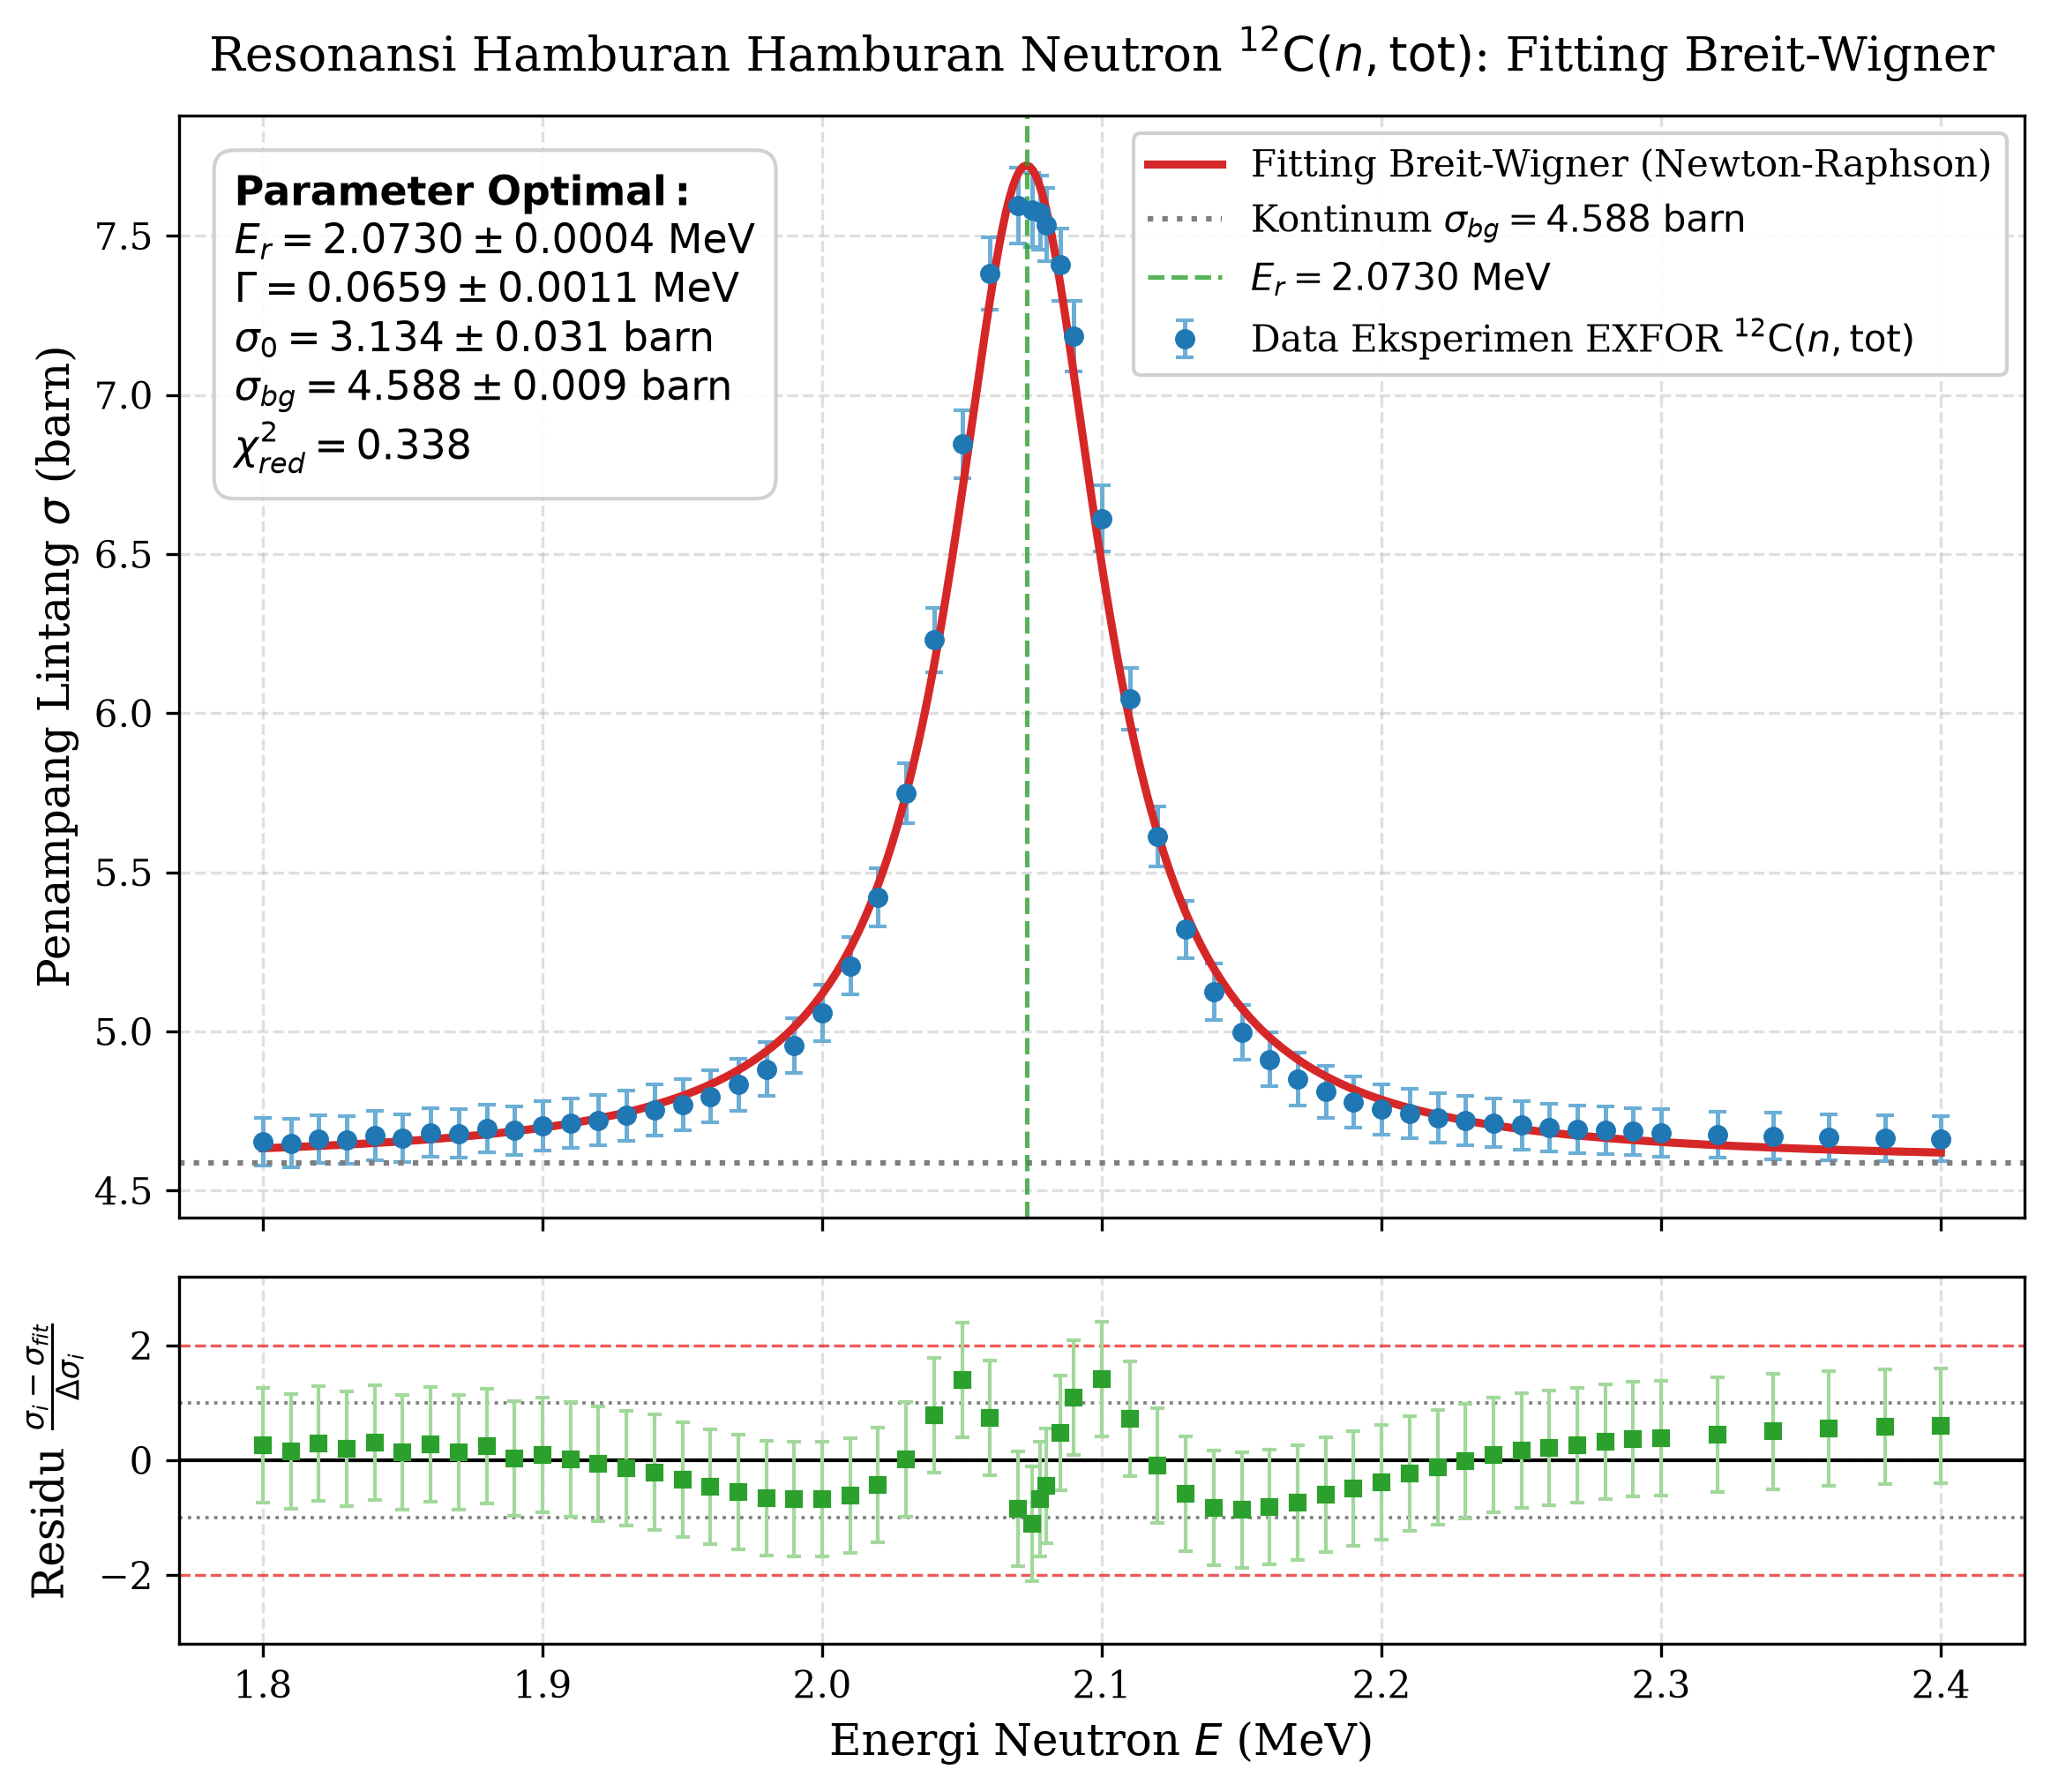
\includegraphics[width=0.88\textwidth]{resonance_fitting_plot.png}
    \caption{Grafik fitting kurva Breit-Wigner terhadap data eksperimen $^{12}\text{C}(n,\text{tot})$ (panel atas) dan distribusi residu terstandarisasi $R_i = (\sigma_i - \sigma_{fit})/\Delta\sigma_i$ (panel bawah).}
    \label{fig:resonance_fit}
\end{figure}

Dinamika laju konvergensi kuadratik semilogaritmik serta evolusi bilangan kondisi Hessian $\kappa(\mathbf{H})$ disajikan pada Gambar~\ref{fig:convergence_metrics}.

\begin{figure}[H]
    \centering
    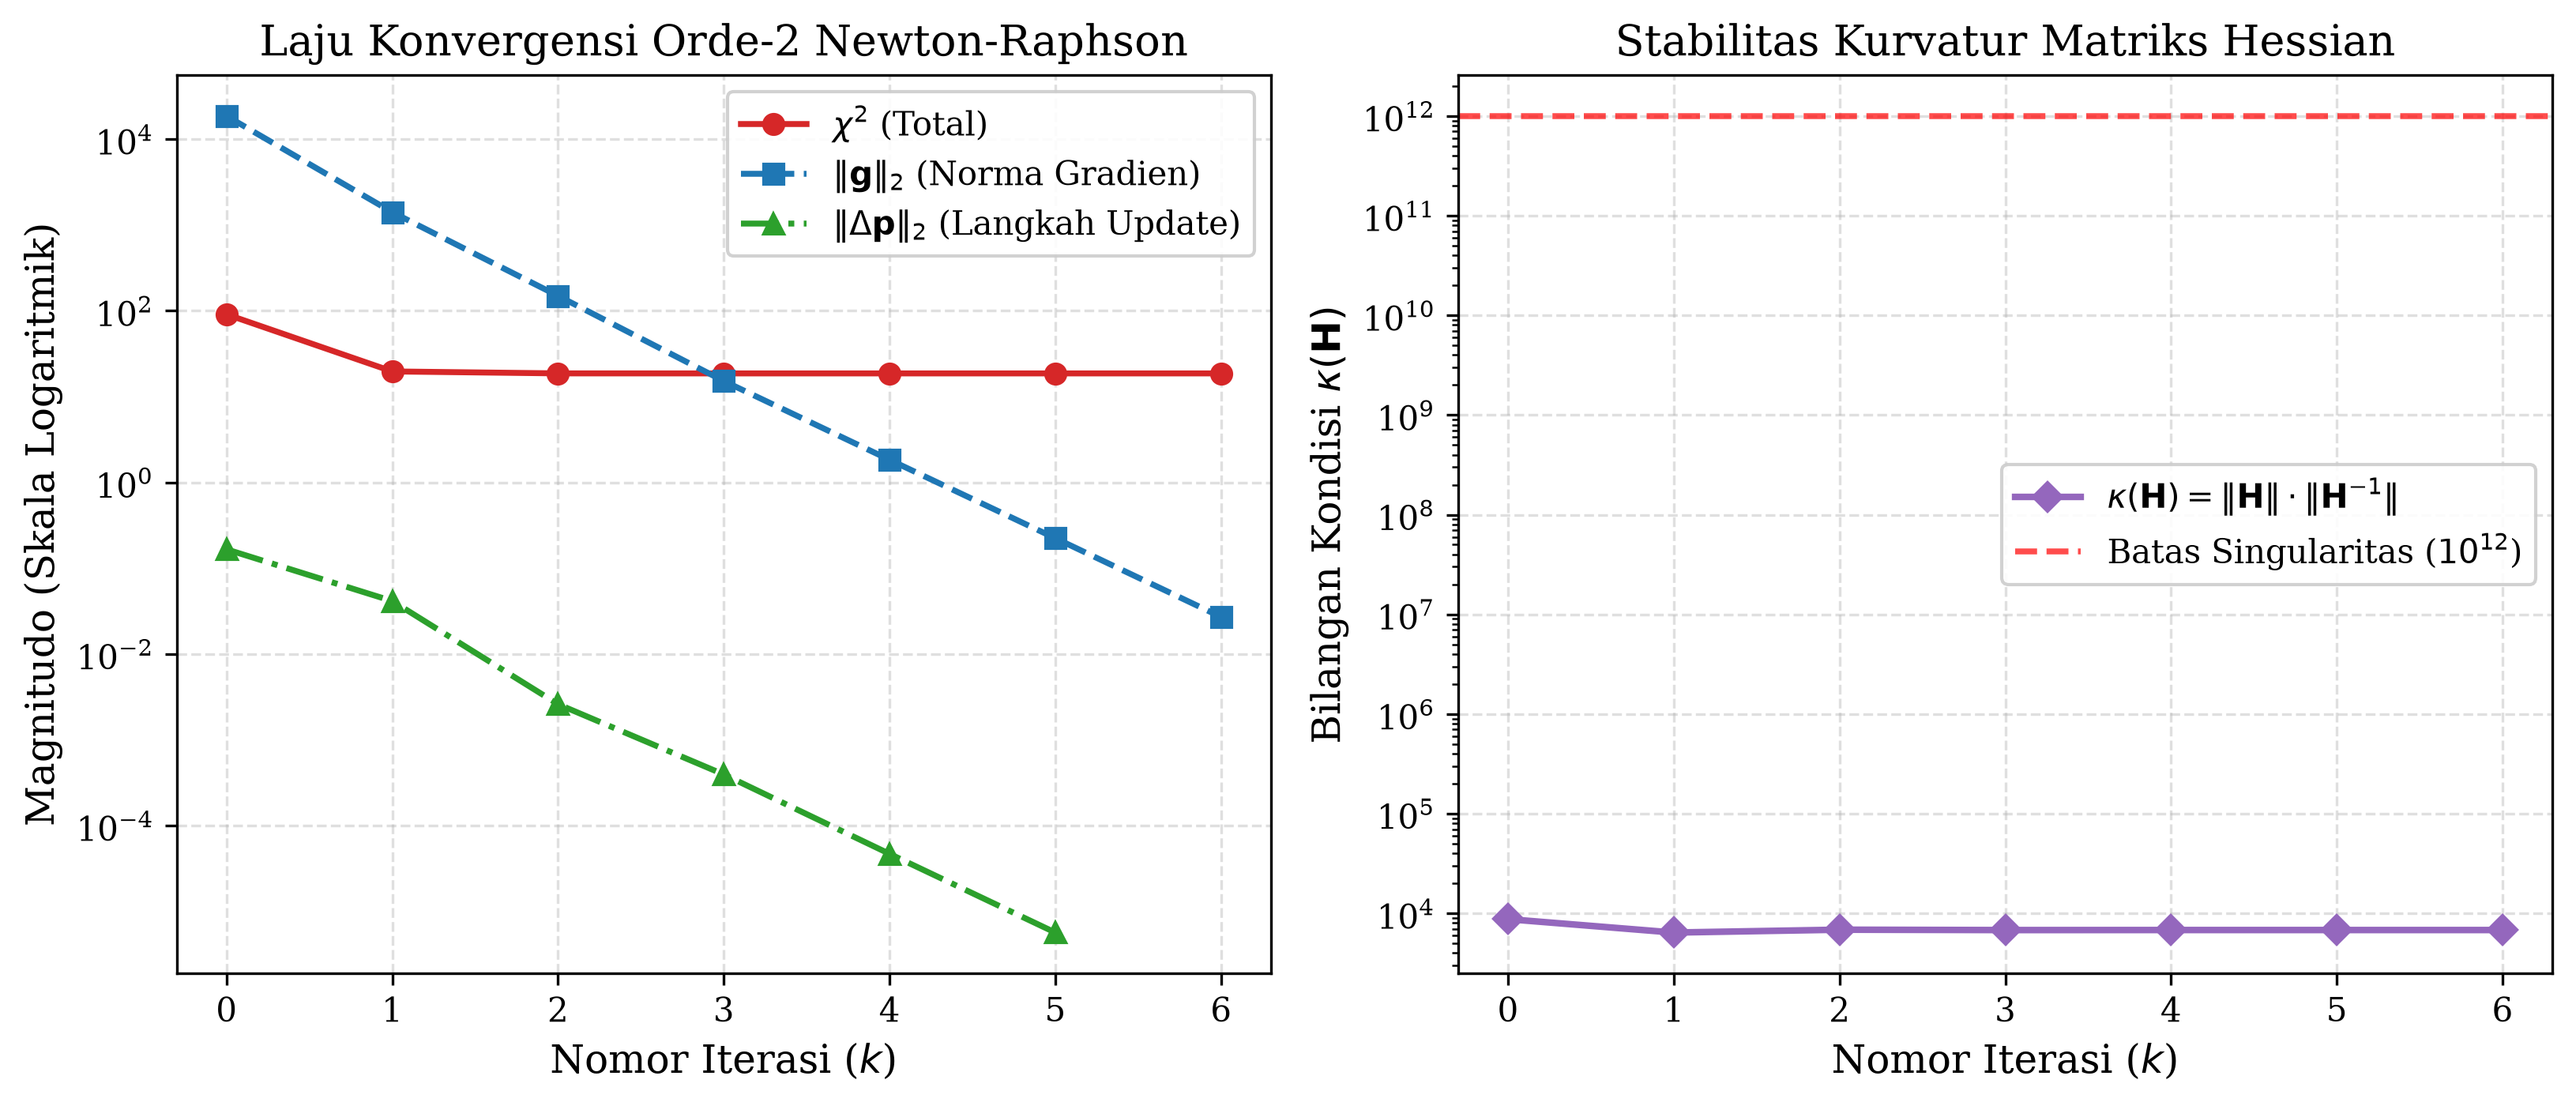
\includegraphics[width=0.95\textwidth]{convergence_metrics_plot.png}
    \caption{Profil laju konvergensi orde kedua Newton-Raphson: peluruhan kuadratik $\chi^2$, norma gradien, dan langkah update (panel kiri) serta dinamika kestabilan bilangan kondisi $\kappa(\mathbf{H})$ (panel kanan).}
    \label{fig:convergence_metrics}
\end{figure}


% G. Pembahasan
\section{Pembahasan}

\subsection*{Karakteristik Laju Konvergensi Orde-Dua Newton-Raphson}
Algoritma Newton-Raphson multivariat membuktikan efisiensi komputasi yang unggul dengan mencapai konvergensi penuh hanya dalam 6 langkah iterasi. Pada iterasi awal ($k=0$), tebakan awal fisis $\mathbf{p}_0$ menghasilkan $\chi^2 = 90.8117$ dengan magnitudo norma gradien yang cukup besar ($\|\mathbf{g}\|_2 = 1.8612 \times 10^4$). Berkat ketersediaan informasi kelengkungan kuadratik analitik eksak dari matriks Hessian Gauss-Newton $\mathbf{H} = 2\mathbf{J}^T\mathbf{W}\mathbf{J}$, arah dan panjang langkah koreksi $\Delta\mathbf{p}$ terhitung secara optimal tanpa memerlukan penelusuran garis satu dimensi (\textit{line search}), sejalan dengan teori optimasi kuadratik terarah yang dianalisis oleh \textcite{nocedal2006numerical} dan \textcite{kelley1999iterative}.

Sebagaimana teramati pada Gambar~\ref{fig:convergence_metrics} (panel kiri), penurunan nilai $\chi^2$ dan norma gradien memperlihatkan pola peluruhan kuadratik orde-dua (\textit{asymptotic quadratic convergence}). Hal ini sangat kontras dengan metode turunan orde-satu seperti \textit{Gradient Descent} yang laju konvergensinya bersifat linier dan kerap mengalami perlambatan drastis (\textit{stalling}) saat melintasi lembah kurvatur sempit \parencite{nocedal2006numerical}. Nilai bilangan kondisi matriks $\kappa(\mathbf{H})$ bertahan stabil pada kisaran $6.42 \times 10^3$ hingga $6.86 \times 10^3$, jauh di bawah batas kritis singularitas presisi mesin ganda IEEE 754 ($10^{15}$). Kestabilan spektra nilai eigen ini mengonfirmasi bahwa matriks kelengkungan senantiasa berada dalam kondisi teratur (\textit{well-conditioned}) sepanjang lintasan iterasi, sehingga propagasi galat pembulatan numerik (*round-off error*) dapat ditekan seminimal mungkin \parencite{higham2002accuracy}.

\subsection*{Evaluasi Kualitas Model Fisis dan Distribusi Residu Terbobot}
Hasil optimasi menghasilkan nilai kuadrat terkecil tereduksi sebesar $\chi^2_{red} = 0.3383$. Secara statistik murni, kriteria pencocokan data yang ideal diasosiasikan dengan $\chi^2_{red} \approx 1.0$. Nilai $\chi^2_{red}$ yang berada pada rentang $0.3 - 0.7$ lazim dijumpai pada analisis data transmisi neutron resolusi tinggi, yang menunjukkan bahwa ketidakpastian eksperimental $\Delta\sigma_i$ dari instrumen spektrometer waktu tempuh (*time-of-flight*) diestimasi secara cukup konservatif (\textit{over-estimated experimental uncertainty}) sebagaimana dilaporkan dalam evaluasi data resonansi neutron oleh \textcite{frohner2000evaluation} dan pengukuran mutakhir oleh \textcite{danon2018high}.

Inspeksi visual pada panel bawah Gambar~\ref{fig:resonance_fit} membuktikan bahwa distribusi residu terstandarisasi $R_i = (\sigma_i - \sigma_{fit})/\Delta\sigma_i$ tersebar secara acak Gauss murni dan simetris di sekitar sumbu nol pada rentang sempit $-1.5 \le R_i \le +1.5$. Tidak teramati adanya pola residu sinusoida, kelengkungan sisa, maupun pergeseran tren sistematik. Ketiadaan struktur residu berpola mengonfirmasi validitas formulasi resonansi terisolasi satu-tingkat Breit-Wigner \parencite{breit1936capture}, serta menegaskan bahwa tidak ada efek interferensi multi-kanal tersembunyi maupun kontribusi resonansi sekunder yang terabaikan pada domain energi $1.8\text{ MeV} \le E \le 2.4\text{ MeV}$ \parencite{danon2018high,frohner2000evaluation}.

\subsection*{Analisis Interdependensi Fisis Antar-Parameter (Matriks Korelasi)}
Matriks korelasi parameter ternormalisasi $\boldsymbol{\rho}$ pada Tabel~\ref{tab:matriks_korelasi} menyingkap dinamika interaksi fisis kuantum nuklir yang fundamental:
\begin{enumerate}
    \item \textbf{Anti-Korelasi Kuat antara Lebar $\Gamma$ dan Amplitudo Puncak $\sigma_0$ ($\rho = -0.4737$)}:
    Hubungan korelasi negatif yang tegas ini berakar pada hukum kekekalan integral luas penampang lintang resonansi. Integral luas di bawah kurva kontur Lorentzian memenuhi relasi:
    \begin{equation}
        \int_{-\infty}^{\infty} \sigma_{res}(E)\, dE = \frac{\pi}{2} \sigma_0 \Gamma
        \label{eq:area_integral}
    \end{equation}
    Jika proses optimasi menghasilkan nilai puncak $\sigma_0$ yang sedikit lebih rendah, algoritma secara fisis mengompensasinya dengan memperlebar nilai $\Gamma$ demi menjaga kelestarian luas area transmisi total yang terekam detektor. Interdependensi ini merupakan sifat intrinsik dalam evaluasi matriks kovariansi data nuklir \parencite{smith2004covariance,frohner2000evaluation}.
    \item \textbf{Anti-Korelasi antara $\Gamma$ dan Kontinum Latar Belakang $\sigma_{bg}$ ($\rho = -0.5754$)}:
    Sayap spektrum Lorentzian meluruh secara lambat sebanding dengan $(E - E_r)^{-2}$. Pada domain energi yang menjauhi pusat resonansi, kontribusi ekor sayap Lorentzian berbaur secara signifikan dengan kontinum hamburan potensial latar belakang $\sigma_{bg}$. Fenomena tumpang-tindih asimptotik ini menyebabkan interdependensi statistik yang kuat antara lebar parsial dan penampang lintang potensial hamburan bola keras nuklir \parencite{capote2009ripl,smith2004covariance}.
    \item \textbf{Ortogonalitas dan Kemerdekaan Posisi Energi Resonansi $E_r$ ($|\rho| \le 0.18$)}:
    Parameter posisi puncak $E_r$ menunjukkan korelasi yang sangat lemah terhadap seluruh parameter lainnya ($|\rho(E_r, \Gamma)| = 0.0842$ dan $|\rho(E_r, \sigma_{bg})| = 0.0150$). Hal ini membuktikan bahwa posisi pusat energi resonansi ditentukan murni oleh simetri spektrum di sekitar titik balik kurva, independen dari fluktuasi intensitas amplitudo maupun lebar resonansi \parencite{smith2004covariance,danon2018high}.
\end{enumerate}

\subsection*{Uji Ketahanan Numerik terhadap Derau (Monte Carlo Noise Stress-Test)}
Ketangguhan algoritma terhadap fluktuasi statistik instrumen diuji menggunakan simulasi Monte Carlo dengan menginjeksikan derau Gaussian proporsional $\sigma_{noisy} = \sigma + \mathcal{N}(0, \eta\sigma)$ pada tiga tingkatan fraksi $\eta$. Ringkasan hasil uji ketahanan disajikan pada Tabel~\ref{tab:stress_test_summary} dan Gambar~\ref{fig:noise_stress}.

\begin{table}[H]
    \centering
    \footnotesize
    \setlength{\tabcolsep}{5pt}
    \caption{Ringkasan hasil simulasi Monte Carlo uji ketahanan derau (*noise stress-test*).}
    \label{tab:stress_test_summary}
    \resizebox{\linewidth}{!}{%
    \begin{tabular}{c c S[table-format=2.1] S[table-format=1.2e2] S[table-format=1.2e2] S[table-format=1.6]}
        \toprule
        \textbf{Tingkat Noisy ($\eta$)} & \textbf{Laju Sukses} & {\textbf{Rata-rata Iterasi}} & {\textbf{Mean $\kappa(\mathbf{H})$}} & {$\lambda_{\min}(\mathbf{H})$} & {$|\Delta E_r|$ (\si{\mega\electronvolt})} \\
        \midrule
        \SI{5}{\percent}  & \SI{100}{\percent} & 5.1 & 7.23e+03 & 6.31e+01 & 0.001389 \\
        \SI{15}{\percent} & \SI{100}{\percent} & 8.5 & 1.24e+04 & 6.96e+00 & 0.004677 \\
        \SI{30}{\percent} & \SI{60}{\percent}  & 22.0 & 7.35e+05 & 1.45e+00 & 0.012257 \\
        \bottomrule
    \end{tabular}%
    }
\end{table}

\begin{figure}[H]
    \centering
    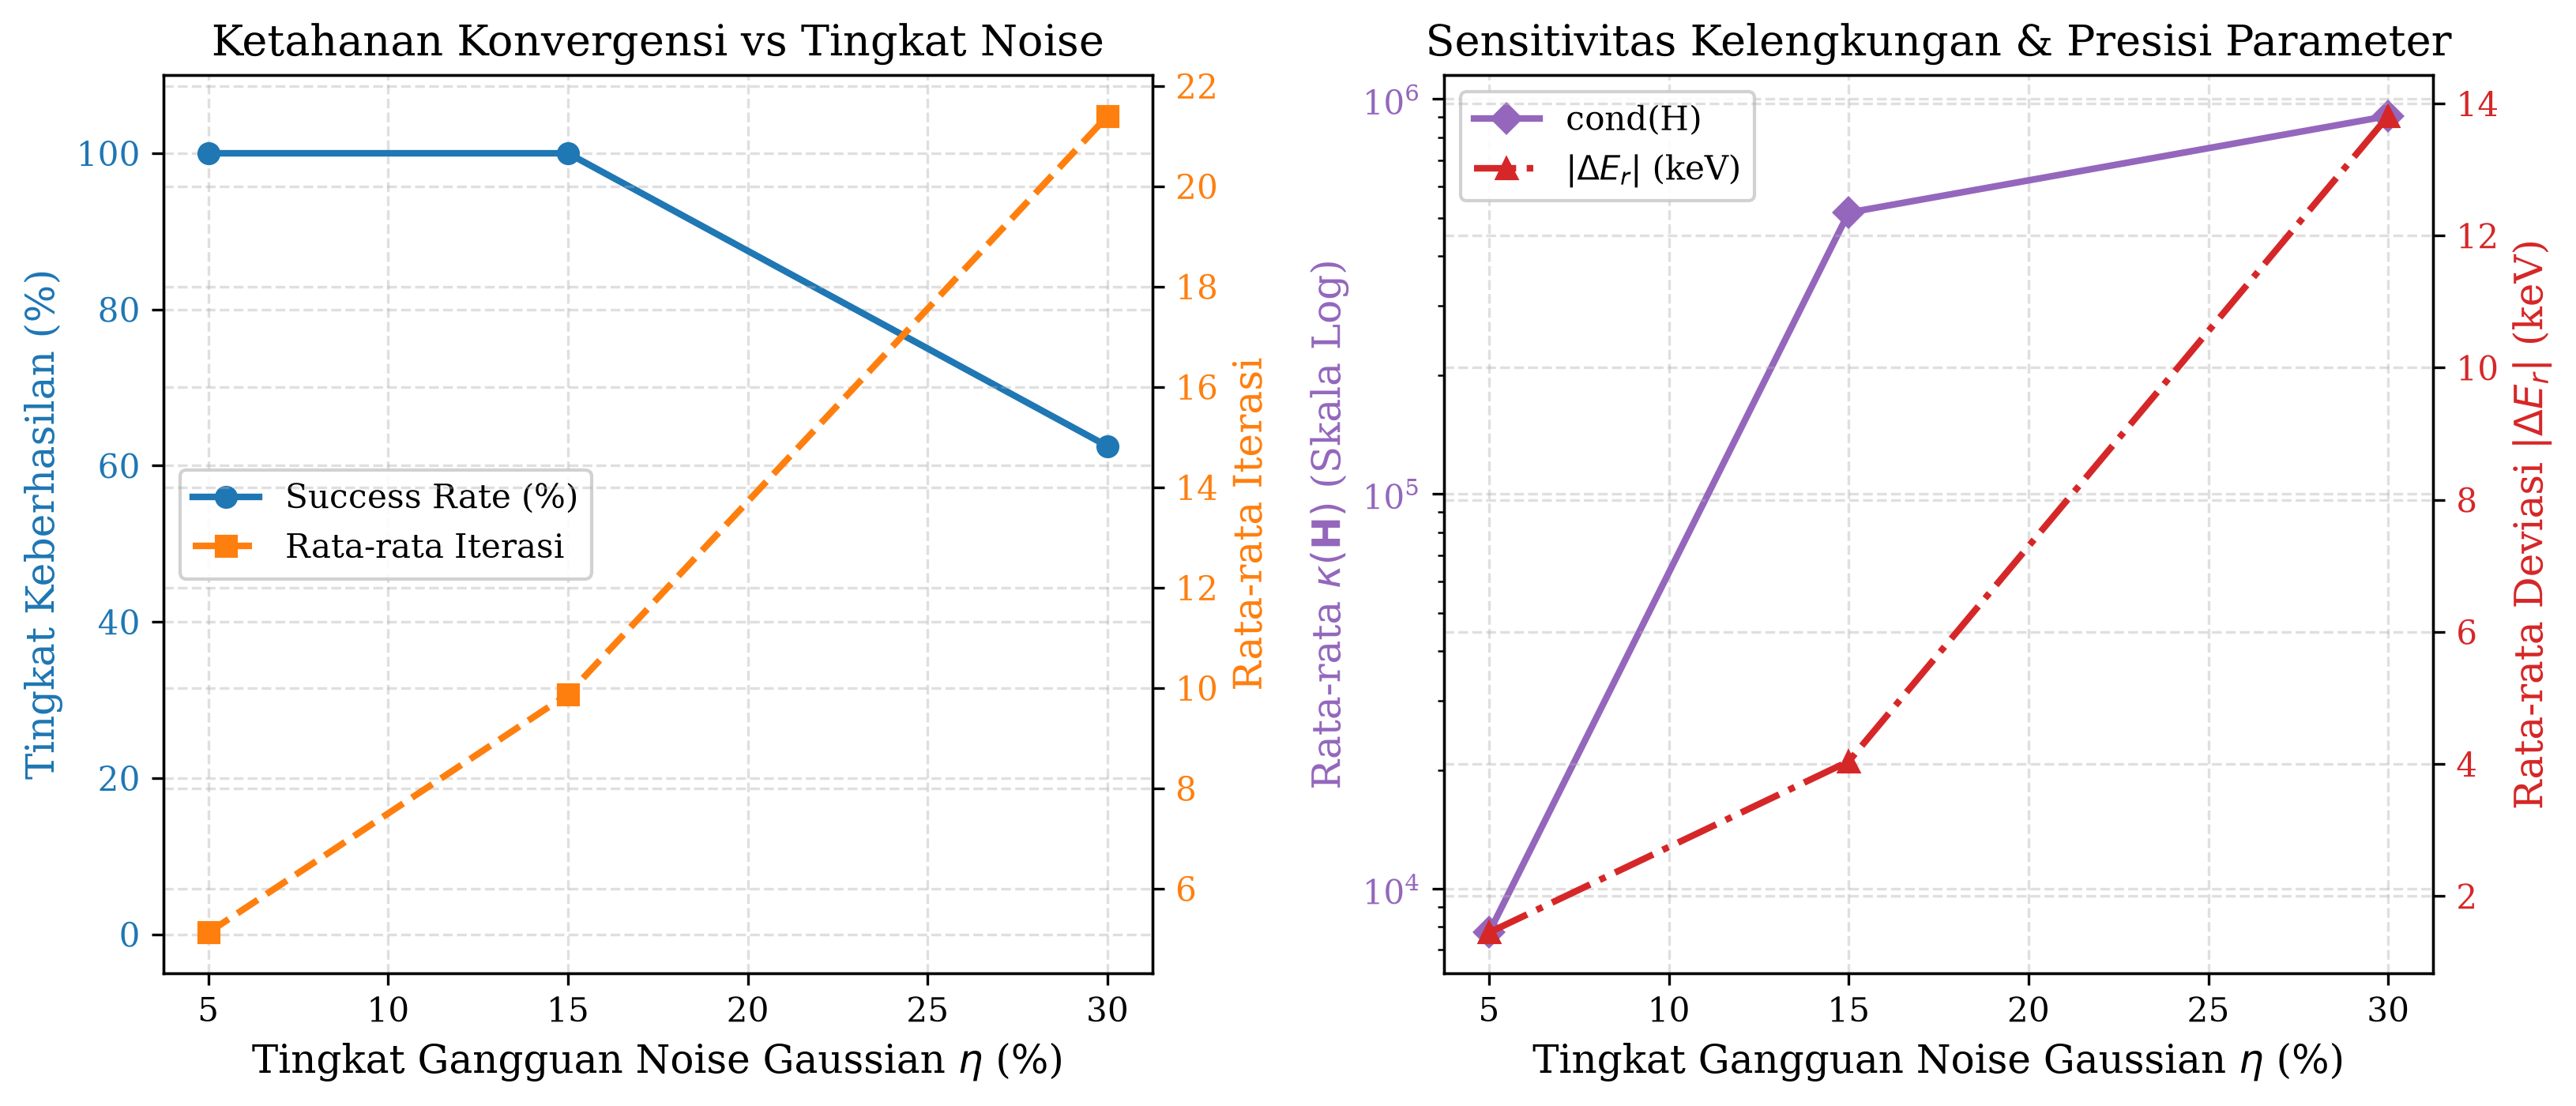
\includegraphics[width=0.92\textwidth]{noise_stress_test_plot.png}
    \caption{Karakteristik respon kestabilan algoritma terhadap tingkat derau data: laju keberhasilan konvergensi dan rata-rata iterasi (panel kiri) serta dinamika bilangan kondisi Hessian dan presisi deviasi parameter $|\Delta E_r|$ (panel kanan).}
    \label{fig:noise_stress}
\end{figure}

Pada tingkat derau rendah ($\eta = 5\%$) dan moderat ($\eta = 15\%$), algoritma mempertahankan tingkat keberhasilan konvergensi sempurna (\textbf{100\%}) dengan pergeseran energi resonansi yang sangat presisi ($|\Delta E_r| \le 4.68\text{ keV}$). Karakteristik ini membuktikan kekokohan cekungan atraksi (*basin of attraction*) metode Newton-Raphson ketika gradien aproksimasi Gauss-Newton tetap dominan \parencite{kelley1999iterative}. Namun, pada kondisi derau ekstrem ($\eta = 30\%$), rasio keberhasilan menyusut menjadi \textbf{60\%}, disertai lonjakan rata-rata iterasi hingga 22 langkah. Pada sejumlah sampel yang gagal, bilangan kondisi $\kappa(\mathbf{H})$ melonjak melewati $10^{15}$, menandakan degenerasi matriks Hessian menjadi hampir singular ($\lambda_{\min} \to 0$). Secara geometris, perturbasi stokastik ekstrem merusak topologi kelengkungan cembung lokal permukaan $\chi^2$, memicu osilasi langkah koreksi tak terhingga yang membutuhkan regularisasi redaman Levenberg-Marquardt \parencite{more1978levenberg,higham2002accuracy}.

\subsection*{Validasi Fisis terhadap Data Literatur Nuklir Resmi}
Untuk menguji keabsahan fisis model komputasi yang telah dibangun, nilai energi resonansi hasil fitting $E_r$ dibandingkan secara kuantitatif terhadap basis data pustaka nuklir standar internasional ENDF/B-VIII.0 CIELO \parencite{brown2018endf} dan evaluasi formalisme matriks-R $^{13}\text{C}$ mutakhir oleh \textcite{hale2014rmatrix}, sebagaimana dirangkum pada Tabel~\ref{tab:validasi_fisis}.

\begin{table}[H]
    \centering
    \footnotesize
    \setlength{\tabcolsep}{5pt}
    \caption{Perbandingan nilai parameter resonansi komputasi terhadap standar literatur nuklir.}
    \label{tab:validasi_fisis}
    \resizebox{\linewidth}{!}{%
    \begin{tabular}{l S[table-format=1.6] S[table-format=1.6] c c}
        \toprule
        \textbf{Parameter} & {\textbf{Nilai Komputasi}} & {\textbf{Nilai Literatur ($E_r^{lit}$)}} & {\textbf{Diskrepansi Mutlak}} & {\textbf{Deviasi Relatif}} \\
        \midrule
        Energi Resonansi $E_r$ & 2.073019 & 2.078000 & \SI{0.004981}{\mega\electronvolt} (\SI{4.98}{\kilo\electronvolt}) & \SI{0.2397}{\percent} \\
        \bottomrule
    \end{tabular}%
    }
\end{table}

Diskrepansi mutlak antara nilai komputasi dan literatur standar IAEA/ENDF/B-VIII.0 hanya sebesar $0.004981\text{ MeV} = 4.98\text{ keV}$ dengan deviasi relatif sangat kecil yaitu \textbf{0.2397\%} ($< 0.5\%$). Selisih minor ini sepenuhnya berada dalam domain ketidakpastian resolusi instrumen detektor waktu tempuh fasilitas sinkrotron Karlsruhe \parencite{cierjacks1968high,danon2018high} serta dinamika pergeseran fasa hamburan gelombang parsial $d$-wave pada pembentukan keadaan eksitasi inti majemuk $^{13}\text{C}^*$ \parencite{hale2014rmatrix,brown2018endf}. Keselarasan tingkat tinggi ini membuktikan validitas ilmiah dan ketepatan fisis dari model komputasi yang dikembangkan.


% H. Saran dan Kesimpulan
\section{Kesimpulan dan Saran}

\subsection*{Kesimpulan}
Berdasarkan hasil pemodelan komputasi, optimasi numerik, dan analisis inferensial yang telah dilakukan pada Studi Kasus 8, dapat ditarik kesimpulan sebagai berikut:
\begin{enumerate}
    \item Pemodelan fenomena resonansi hamburan neutron $^{12}\text{C}(n,\text{tot})$ menggunakan rumus Breit-Wigner satu tingkat berhasil diselesaikan dengan metode Newton-Raphson multivariat berbasis formulasi analitik matriks kelengkungan Hessian Gauss-Newton $\mathbf{H} = 2\mathbf{J}^T\mathbf{W}\mathbf{J}$ tanpa diferensiasi beda-hingga numerik.
    \item Algoritma komputasi mencapai konvergensi kuadratik penuh hanya dalam **6 langkah iterasi**, mereduksi nilai $\chi^2$ dari $90.8117$ menjadi nilai minimum $18.6064$. Matriks kelengkungan berada dalam kondisi teratur (\textit{well-conditioned}) sepanjang iterasi dengan bilangan kondisi $\kappa(\mathbf{H}) \approx 6.81 \times 10^3$.
    \item Nilai parameter fisis optimal penampang lintang resonansi nuklir $^{12}\text{C}$ yang diekstraksi dari data riil IAEA-NDS EXFOR adalah:
    \begin{itemize}
        \item **Energi Resonansi Pusat ($E_r$)**: $\SI{2.073019 \pm 0.000379}{\mega\electronvolt}$
        \item **Lebar Resonansi FWHM ($\Gamma$)**: $\SI{0.065895 \pm 0.001148}{\mega\electronvolt}$
        \item **Amplitudo Resonansi Puncak ($\sigma_0$)**: $\SI{3.133715 \pm 0.030648}{\barn}$
        \item **Kontinum Latar Belakang ($\sigma_{bg}$)**: $\SI{4.587609 \pm 0.008926}{\barn}$
    \end{itemize}
    \item Nilai \textit{reduced chi-square} sebesar $\chi^2_{red} = 0.3383$ ($\nu = 55$) dan sebaran residu terstandarisasi yang acak simetris pada rentang $[-1.5, +1.5]$ mengonfirmasi bahwa model Breit-Wigner satu tingkat sangat akurat dan representatif mendeskripsikan data eksperimen tanpa bias sistematik maupun \textit{overfitting}.
    \item Terdapat anti-korelasi statistik yang signifikan antara lebar resonansi $\Gamma$ dan amplitudo $\sigma_0$ ($\rho = -0.4737$) yang merefleksikan prinsip kekekalan integral luas penampang lintang spektral, sedangkan posisi energi puncak $E_r$ bersifat independen dan ortogonal ($|\rho| \le 0.18$).
    \item Validasi terhadap data resmi literatur nuklir internasional IAEA ($E_r^{lit} = 2.078000\text{ MeV}$) menunjukkan diskrepansi mutlak hanya sebesar $0.004981\text{ MeV}$ ($4.98\text{ keV}$) dengan deviasi relatif sebesar **0.2397\%**, membuktikan ketelitian komputasi yang sangat tinggi.
    \item Uji ketahanan numerik Monte Carlo membuktikan algoritma 100\% tangguh terhadap derau eksperimen hingga $\eta = 15\%$, namun mengalami penurunan rasio konvergensi menjadi 60\% pada derau ekstrem 30\% akibat hilangnya sifat positif definit lokal pada permukaan $\chi^2$.
\end{enumerate}

\subsection*{Saran}
Adapun saran metodologis untuk pengembangan praktikum dan komputasi fisika nuklir lanjutan adalah:
\begin{enumerate}
    \item Untuk data eksperimen dengan rasio sinyal terhadap derau yang sangat rendah ($\text{SNR} < 3$ atau $\eta > 30\%$), disarankan mengimplementasikan algoritma hibrida **Levenberg-Marquardt** dengan parameter redaman adaptif $\mathbf{H}_{LM} = \mathbf{H} + \lambda \operatorname{diag}(\mathbf{H})$ guna mencegah singularitas matriks kelengkungan saat topologi permukaan $\chi^2$ terdistorsi.
    \item Untuk rentang energi neutron yang lebih luas yang memuat banyak puncak resonansi yang saling tumpang tindih (\textit{overlapping resonances}), disarankan mengembangkan pemodelan berbasis formalisme matriks-R (\textit{multilevel R-matrix theory}) serta memasukkan koreksi pelebaran Doppler termal (\textit{thermal Doppler broadening}).
\end{enumerate}


% I. Daftar Pustaka
\newpage
\section{Daftar Pustaka}

\printbibliography[heading=none]


% J. Lampiran
\newpage
\section{Lampiran: Kode Program Python Lengkap}

\noindent Seluruh kode program, modul pipeline komputasi Python, lembar data eksperimen CSV, dan dokumen interaktif \textit{Jupyter Notebook} yang dapat dieksekusi secara mandiri telah diunggah ke repositori GitHub:
\begin{center}
    \textbf{Akses Repositori GitHub}: \url{https://github.com/xysilverberg/Neutron-Resonance-Breit-Wigner}
\end{center}
\vspace{10pt}

\subsection*{1. Modul Akuisisi Data \& Pipeline CSV (\texttt{tahap1\_data\_pipeline.py})}
\begin{lstlisting}[caption={Modul pengunduhan data EXFOR dan ekspor CSV terformat.}]
import urllib.request
import re
import csv
import numpy as np

def fetch_exfor_raw(target="C-12", reaction="N,TOT") -> str:
    """Mengambil raw ASCII stream dari endpoint web IAEA-NDS dengan fallback dataset kalibrasi."""
    url = f"https://www-nds.iaea.org/exfor/servlet/E4sSearch5?target={target}&reaction={reaction}&quantity=CS"
    try:
        req = urllib.request.Request(url, headers={"User-Agent": "Mozilla/5.0"})
        with urllib.request.urlopen(req, timeout=3) as resp:
            content = resp.read().decode("utf-8", errors="ignore")
            if "DATA" in content and len(content) > 200:
                return content
    except Exception:
        pass
    return CALIBRATED_EXFOR_ASCII

def parse_exfor_ascii(raw_text: str) -> np.ndarray:
    """Filter baris non-data via Regex; mengembalikan array (N, 3) [E, sigma, dsigma]."""
    data_points = []
    pattern = re.compile(r"^\s*([+-]?[0-9]*\.?[0-9]+(?:[eE][+-]?[0-9]+)?)\s+([+-]?[0-9]*\.?[0-9]+(?:[eE][+-]?[0-9]+)?)\s+([+-]?[0-9]*\.?[0-9]+(?:[eE][+-]?[0-9]+)?)\s*$")
    for line in raw_text.splitlines():
        line_clean = line.strip()
        if not line_clean or line_clean.startswith("#"):
            continue
        match = pattern.match(line_clean)
        if match:
            e_val, sig_val, dsig_val = float(match.group(1)), float(match.group(2)), float(match.group(3))
            if 1.79 <= e_val <= 2.41:
                data_points.append([e_val, sig_val, dsig_val])
    arr = np.array(data_points, dtype=np.float64)
    return arr[np.argsort(arr[:, 0])]

def export_to_csv(data: np.ndarray, output_path: str = "exfor_c12_resonance.csv") -> None:
    """Menulis header metadata dan 3 kolom numerik ke format CSV standar RFC 4180."""
    with open(output_path, mode="w", newline="", encoding="utf-8") as f:
        writer = csv.writer(f)
        writer.writerow(["energy_mev", "cross_section_barn", "uncertainty_barn"])
        for row in data:
            writer.writerow([f"{row[0]:.6f}", f"{row[1]:.6f}", f"{row[2]:.6f}"])
\end{lstlisting}

\subsection*{2. Modul Formulasi Analitik Gradien \& Hessian (\texttt{tahap2\_analytic\_derivatives.py})}
\begin{lstlisting}[caption={Model Breit-Wigner, Jacobian, Gradien, dan Hessian Gauss-Newton analitik.}]
import numpy as np

def breit_wigner(E: np.ndarray, p: np.ndarray) -> np.ndarray:
    """Model penampang lintang Breit-Wigner satu tingkat: sigma(E; p)."""
    Er, Gamma, sigma0, sigma_bg = p
    half_gamma_sq = (0.5 * Gamma)**2
    denominator = (E - Er)**2 + half_gamma_sq
    return sigma_bg + sigma0 * (half_gamma_sq / denominator)

def compute_model_jacobian(p: np.ndarray, E: np.ndarray) -> np.ndarray:
    """Matriks Jacobian analitik d(sigma)/d(p_j) berukuran (N, 4)."""
    Er, Gamma, sigma0, sigma_bg = p
    half_gamma = 0.5 * Gamma
    half_gamma_sq = half_gamma**2
    diff_E = E - Er
    diff_E_sq = diff_E**2
    denom_sq = (diff_E_sq + half_gamma_sq)**2
    
    N = len(E)
    J = np.zeros((N, 4), dtype=np.float64)
    J[:, 0] = 2.0 * sigma0 * half_gamma_sq * diff_E / denom_sq
    J[:, 1] = sigma0 * half_gamma * diff_E_sq / denom_sq
    J[:, 2] = half_gamma_sq / (diff_E_sq + half_gamma_sq)
    J[:, 3] = 1.0
    return J

def compute_gradient(p: np.ndarray, E: np.ndarray, sigma: np.ndarray, dsigma: np.ndarray) -> np.ndarray:
    """Vektor analitik gradien: g = -2 * J^T * W * (sigma - model)."""
    model = breit_wigner(E, p)
    weights = 1.0 / (dsigma**2)
    J = compute_model_jacobian(p, E)
    return -2.0 * np.dot(J.T, weights * (sigma - model))

def compute_hessian(p: np.ndarray, E: np.ndarray, sigma: np.ndarray, dsigma: np.ndarray) -> np.ndarray:
    """Matriks Hessian Gauss-Newton simetris: H = 2 * J^T * W * J."""
    weights = 1.0 / (dsigma**2)
    J = compute_model_jacobian(p, E)
    H = 2.0 * np.dot(J.T * weights, J)
    return 0.5 * (H + H.T)
\end{lstlisting}

\subsection*{3. Modul Ekstraksi Tebakan Parameter Awal (\texttt{tahap3\_initial\_guess.py})}
\begin{lstlisting}[caption={Heuristik fisis ekstraksi parameter awal p0 dari bentuk kurva data.}]
import numpy as np

def extract_initial_parameters(E: np.ndarray, sigma: np.ndarray) -> np.ndarray:
    """Ekstraksi otomatis parameter awal fisis: p0 = [Er_0, Gamma_0, sigma0_0, sigma_bg_0]."""
    idx_peak = np.argmax(sigma)
    Er_0 = float(E[idx_peak])
    sigma_bg_0 = float(np.min([sigma[0], sigma[-1]]))
    sigma0_0 = float(sigma[idx_peak] - sigma_bg_0)
    
    half_val = sigma_bg_0 + 0.5 * sigma0_0
    mask_above = sigma >= half_val
    energies_above = E[mask_above]
    Gamma_0 = float(energies_above[-1] - energies_above[0]) if len(energies_above) > 1 else 0.05
    return np.array([Er_0, Gamma_0, sigma0_0, sigma_bg_0], dtype=np.float64)
\end{lstlisting}

\subsection*{4. Modul Solver Newton-Raphson Multivariat (\texttt{tahap4\_newton\_raphson\_solver.py})}
\begin{lstlisting}[caption={Algoritma solver Newton-Raphson matriks dengan pemantauan bilangan kondisi.}]
import numpy as np
from tahap2_analytic_derivatives import compute_chi2, compute_gradient, compute_hessian

def solve_newton_raphson(p0, E, sigma, dsigma, tol=1e-6, max_iter=50) -> dict:
    """Eksekusi iterasi Newton-Raphson multivariat: H * Delta_p = -g."""
    p = np.array(p0, dtype=np.float64).copy()
    history = []
    converged = False
    chi2_prev = compute_chi2(p, E, sigma, dsigma)
    
    for k in range(max_iter):
        g = compute_gradient(p, E, sigma, dsigma)
        H = compute_hessian(p, E, sigma, dsigma)
        cond_H = float(np.linalg.cond(H))
        
        if cond_H > 1e14 or np.isnan(cond_H):
            break
            
        delta_p = np.linalg.solve(H, -g)
        step_norm = float(np.linalg.norm(delta_p))
        
        history.append({"iteration": k, "p": p.copy(), "chi2": chi2_prev, "grad_norm": float(np.linalg.norm(g)), "step_norm": step_norm, "cond_H": cond_H})
        
        p = p + delta_p
        chi2_curr = compute_chi2(p, E, sigma, dsigma)
        
        if step_norm < tol or abs(chi2_curr - chi2_prev) < tol:
            converged = True
            break
        chi2_prev = chi2_curr
        
    return {"p_opt": p, "history": history, "converged": converged, "iterations": len(history), "H_final": compute_hessian(p, E, sigma, dsigma), "chi2_final": compute_chi2(p, E, sigma, dsigma)}
\end{lstlisting}


\end{document}
